\documentclass[12pt]{jarticle} 
\usepackage[top=20truemm,bottom=20truemm,left=20truemm,right=20truemm]{geometry}
\usepackage[dvipdfmx]{graphicx}
\usepackage{ascmac}
\usepackage{amsfonts}
\usepackage{amsthm}
\usepackage{comment}
\usepackage{type1cm}
\usepackage{bm}
\usepackage{amsmath, amssymb}
\usepackage{listings,jlisting}
\usepackage{algorithm,algorithmic}
\usepackage{cases}
\lstset{language=C,
        basicstyle=\footnotesize,
        commentstyle=\textit,
        classoffset=1,
        keywordstyle=\bfseries,
	frame=tRBl,framesep=5pt,
	showstringspaces=false,
        numbers=left,stepnumber=1,numberstyle=\footnotesize,
	breaklines=true
	}
%\usepackage{igo}
\thispagestyle{empty}
\def\mathbfit#1{\mbox{\mathversion{bold}$#1$\mathversion{normal}}}
\def\C{\mathbb{C}}
\def\R{\mathbb{R}}
\def\N{\mathbb{N}}
\def\Z{\mathbb{Z}}
\def\PROBLEM#1{\ifmmode{\langle #1 \rangle}\else\ifinner{\langle #1 \rangle}
        \else{$\langle #1 \rangle$}\fi\fi}
\def\SET#1#2{\left\{#1 : #2\right\}}
\def\bx{\mathbfit{x}}
\def\by{\mathbfit{y}}
\def\bg{\mathbfit{g}}
\def\bb{\mathbfit{b}}
\def\bp{\mathbfit{p}}
\def\bq{\mathbfit{q}}
\def\br{\mathbfit{r}}
\def\b0{\mathbfit{0}}
\def\mN{\mathcal{N}}
\def\mP{\mathcal{P}}
\def\mV{\mathcal{V}}
\def\norm<#1>{\langle #1 \rangle}
\newcommand{\argmax}{\mathop{\rm arg~max}\limits}
\newcommand{\argmin}{\mathop{\rm arg~min}\limits}

\begin{document}
\thispagestyle{empty}
\vfill
\hfill 電気通信大学情報理工学研究家 \\
\hfill 情報・ネットワーク工学専攻情報数理工学コース修士論文
%
%\hfill 電気通信大学電気通信学部 \\
%\hfill 情報工学科卒業論文
%
%\hfill 電気通信大学情報理工学部 \\
%\hfill 先端工学基礎課程卒業論文
\vfill
\begin{center}
  \Large 集中ノードの存在を考慮したライトニングネットワークのルーティング問題
\end{center}
\vfill
\begin{center}
  \today
\end{center}
\vfill
\begin{center}
  \large
  情報数理工学コース\\[1cm]
  学籍番号 1831111\\[1cm]
  中村大地
\end{center}
\begin{center}
  
\end{center}
\vfill
\pagebreak

\section{はじめに}
近年、ブロックチェーン\cite{satoshi}と呼ばれる分散型元帳技術を活用したサービスやアプリケーションが世界中で注目を集めている。ブロックチェーンとは2009年にサトシ・ナカモト\cite{satoshi}によって発表された電子マネーシステムの根幹となる分散型元帳技術である。ハッシュ関数による暗号化を使用することで、従来の金融システムにおける銀行や造幣局と言った管理者が存在しない非管理・非中央集権型のネットワークにおいて信頼できる取引を行うことができるシステムである。2019年6月時点でブロックチェーンの技術を使用した仮想通貨が2200種類を超え、最も有名なBitcoinでは時価総額が17兆円を超えるほどの規模となっている\cite{coin}。
\par
一方、ブロックチェーンは元帳システムとしては有用な性質を持っているが支払いシステムとしては重大な問題を抱えている。それがスケーラビリティ、単位時間当たりに処理できる取引数である。金融決済システムVISAではピーク時に秒間56000取引の処理を記録したが、ビットコインでは2017年時点で1秒間に7取引しか処理することができなかった\cite{joseph}。これは支払いシステムとしてだけではなく元帳システムとしても重大な問題である。2019年6月現在ビットコインシステムでは作成されてからチェーンに追加されるのを待っている保留トランザクションが約20000個存在している。
\par
このスケーラビリティ問題を解決する方法として2016年にJosephら\cite{joseph}によって提案されたライトニングネットワークが注目されている。ライトニングネットワークは取引をブロックチェーン外のマイクロペイメントチャネルで処理し、チャネルの開設と閉鎖のみをブロックチェーンに記録することで取引の高速化、及びトランザクションの削減を目指す。さらにライトニングネットワークでは直接チャネルを開設していないユーザ同士であってもチャネルを開設している別のユーザを経由することで送金を行うことを可能にした。他のユーザを経由して送金を行うためにはどのユーザを経由して送金を行うかを決定するルーティングが必要となるが、ライトニングネットワークではこのルーティングにまだ課題を抱えている。
本稿はPavelら\cite{flare}によって提案されたライトニングネットワークのルーティングアルゴリズム「Flare」に関して、その拡張と課題の解決を目的とする。

\section{ブロックチェーン}
ブロックチェーンとは2009年にサトシ・ナカモト\cite{satoshi}によって発表された改竄が困難な分散型元帳を作成する技術である。改竄が困難でありかつ特定の管理ノードが存在せず耐故障性に優れているという性質から近年注目を集めている。代表的な使用例としてビットコインをはじめとする仮想通貨が存在する。
\par
ブロックチェーンにはそれを使用するユーザと、ユーザ同士の繋がりによってできるネットワークが存在することが前提である。このネットワークをブロックチェーンネットワークと呼ぶ。一般的にブロックチェーンネットワークにおいてノードはネットワークに参加しているユーザを意味し、エッジはユーザ同士の接続を表す。ブロックチェーンネットワークはP2Pに分類されるネットワークであり、参加するユーザ同士が相互に情報のやり取りを行なっている。また特定の管理ノードが存在せず、ネットワークの一部が故障しても全体のパフォーマンスに大きな影響を与えないことから耐故障性に優れていると言われている。
\par
ブロックチェーンネットワークに参加するユーザはフルノードとSimplified Payment Verification(SPV)ノードの2種類に分類される。フルノードとはブロックチェーンに記録されたデータ全てを自身の端末上に保管しているノードである。全ての取引の記録を持っていることから、過去の取引のデータを参照し新しい取引の検証を行ったり、ブロックチェーン全体の整合性を確認することができる。しかし、近年ブロックチェーンに参加するユーザ数が増加したことによりブロックチェーン自体の容量が大幅に増加し、全ての記録を保持できないノードが現れ始めた。そこで導入されたのがSPVノードである。これはブロックチェーンに記録されたデータの一部しか保持しない代わりに取引の検証やブロックチェーンの整合性の確認ができなくなったノードである。検証は行えないがブロックチェーンの使用はできることから近年このSPVノードが増えている。

\section{ブロックチェーンの暗号化技術}
ブロックチェーンの大きな特徴として改竄が困難であるというものがある。これを実現しているのがブロックチェーンの暗号化技術である。ブロックチェーンの最も一般的な暗号化方式としてハッシュ関数と楕円曲線暗号の組み合わせがある。楕円曲線暗号とは公開鍵暗号の一種である。ブロックチェーンでは楕円曲線暗号の中でも特にsecp256k1と呼ばれるNIST(米国標準技術局)が定義した特別な楕円曲線を使用している。

\subsection{ハッシュ関数}
ハッシュ関数とは、入力した値に対して全く別の値を返す関数のことである。この関数の返り値をハッシュ値と呼ぶ。ハッシュ関数は以下のような性質を持つ。

\begin{itemize}
\item 同じ値を入力すれば必ず同じハッシュ値を返す
\item 入力した値が1ビットでも異なればハッシュ値も全く異なる値になる
\item ハッシュ値から入力した値を推定することが困難(不可逆性)
\item ハッシュ値の長さは入力した値の長さによらず一定
\item 入力が異なる場合、同じハッシュ値を返すことは原則としてない
\end{itemize}

\begin{figure}[h]
 \centering
   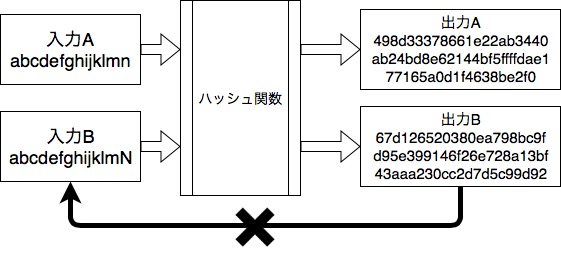
\includegraphics[width=80mm]{figures/hash.jpg}
 \caption{ハッシュ関数によるハッシュ値の計算}
 \label{tree1}
\end{figure}

このハッシュ関数を用いた暗号化と検証の仕組みによってブロックチェーン上でのデータの改竄は困難となっている。ブロックチェーンにおけるデータの検証の仕組みを図\ref{check}に示す。

\begin{figure}[h]
 \centering
   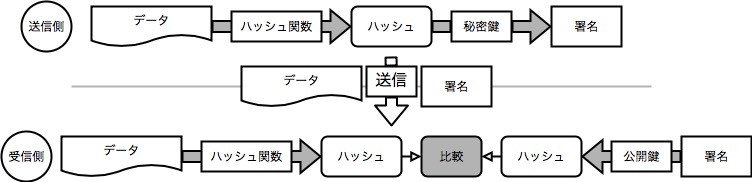
\includegraphics[width=120mm]{figures/signature-2.jpg}
 \caption{ハッシュ関数を用いた検証}
 \label{check}
\end{figure}

送信者は送信するデータをハッシュ関数に入力することによってハッシュ値を計算し、計算したハッシュ値と自身の秘密鍵を用いて署名を作成する(図\ref{check}上)。そしてデータと署名を受信者に送信し検証を行ってもらう。受信側は送られたデータをハッシュ関数に入力することによって再度ハッシュ値を計算し、さらに署名に対して送信者の公開鍵を用いて元のハッシュ値を復号する。この再度計算したハッシュ値と署名から復号したハッシュ値を比較することで送信されたデータの検証が行える(図\ref{check}下)。この検証によって受信者は以下の項目を確認することができる。

\begin{itemize}
\item 送られたデータの送信者が正しいのか
	\begin{itemize}
	\item 送信者が正しくなければ公開鍵を用いての署名の復号が行えないため
	\end{itemize}
\item 送信されたデータが途中で改竄されていないか
	\begin{itemize}
	\item 途中でデータが改竄されていた場合受信者が計算し直したハッシュ値と署名から復号したハッシュ値が一致しないため
	\end{itemize}
\end{itemize}

改竄の検出の例として、送信途中で攻撃者によりデータが改竄されたとする。この時受信側には攻撃者によって改竄された偽のデータと送信者が作成した署名が送られる。この時も受信者はハッシュ値の計算と署名の復号を行いその結果を比較するが、偽データから作られる偽のハッシュ値と送信者の公開鍵によって復号された正しいデータから作られたハッシュ値はハッシュ関数の性質により異なるものとなる。これにより受信者は受け取ったデータが改竄されたものであると気づくことができる。

\begin{figure}[h]
 \centering
   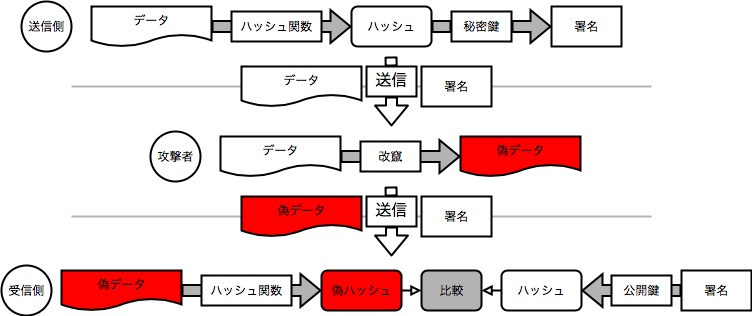
\includegraphics[width=120mm]{figures/signature-attack.jpg}
 \caption{送信途中での改竄の検出}
 \label{attack}
\end{figure}

このようにブロックチェーンに記録されるデータはハッシュ関数によって暗号化、検証され、データの対となるハッシュ値は公開鍵を用いたデジタル署名がされることで安全かつ確実なデータのやり取りを可能にしている。


\section{ビットコイン}
ビットコインとはブロックチェーン技術を使用した仮想通貨の1種類である。通貨単位はBTC、あるいはsatoshiであり、1satoshi = 0.00000001BTCである。2019年9月時点において1BTC=\$10,415.36となっている。2019年時点において世界で最も普及している仮想通貨であり、利用しているユーザ数は1000万人、時価総額は22兆円と言われている。しかし、ビットコインは幅広く普及している一方で多くの事件を起こし、様々な課題を抱えている。仮想通貨に関わる代表的な事件として以下のようなものがある。

\begin{itemize}
\item 2019年7月 BITponitがハッキングを受け30億円相当の仮想通貨が流出\cite{jiken1}
\item 2018年2月 BitGrailから仮想通貨「Nano」が流出。約211億円の被害が生じた\cite{jiken2}
\item 2018年1月コインチェックが保有していた仮想通貨「NEM」がクラッキングにより流出。約580億円の被害が生じた\cite{jiken3}
\item 2016年6月 自律分散型投資ファンド「The DAO」がシステムの脆弱性をつかれ約43億円のEthereumが流出\cite{jiken4}
\end{itemize}

これらの事件はその金額の大きさから社会的にも非常に大きな影響を与えた。ビットコインをはじめとした仮想通貨ではこれらの問題の解決による安全性の向上、及び使用上の利便性を向上させるための研究が活発に行われている。本章では仮想通貨「ビットコイン」について、その仕様や現在問題視されている課題について解説する。

\subsection{ウォレット}
ビットコインでは、各ユーザは銀行における口座に相当するウォレットを所持している。ユーザはこのウォレットを通じて自身の所持金を管理・運用していく。そしてユーザとウォレット、ウォレットと資産を紐づけるものが秘密鍵と公開鍵である。この秘密鍵と公開鍵が資産を管理する上での鍵と錠の役目を担っている。
\\
全てのユーザはビットコインの使用を開始した時点で自動で秘密鍵と公開鍵を振り分けられる。そして公開鍵をエンコードしたアドレスを与えられ、そのアドレスを使用して資産の送金や受取を行う。このアドレスを介した資産のやり取りにおいて、資産を受け取った時に他人に資産を勝手に使用されないように受信者の公開鍵でロックをかける。これが公開鍵の錠としての役目である。自身の資産を利用したいときは、公開鍵によって施したロックを外す。このロックを外すのが最初に振り分けられた秘密鍵の鍵としての役目である。
\par
ユーザは秘密鍵・公開鍵とウォレットを利用して自身の資産を管理・運用するが、ウォレットに直接資産が保管されているわけではない。ウォレットに保管されているのはユーザの秘密鍵である。資産としてのビットコインはユーザのウォレット内には保管されず、全てブロックチェーンに記録される台帳に存在している。ブロックチェーンに記録されている取引の中で自身が最後に受け取り、公開鍵を用いて錠をした後に一度も使用していない取引の合計金額がビットコインにおける残高である。ユーザは公開鍵における錠とウォレットに保管した秘密鍵を紐づけることでブロックチェーン上に存在する自身の残高を管理する。

\begin{figure}[h]
 \centering
   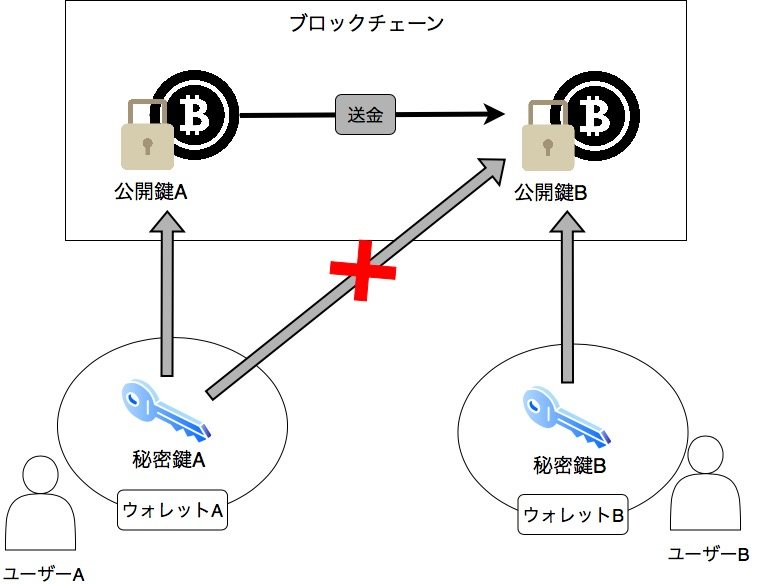
\includegraphics[width=80mm]{figures/wallet.jpg}
 \caption{ウォレットによる資産の管理}
 \label{wallet}
\end{figure}

つまり、ビットコインにおける資産の移動とは自身の資産に対して自身の秘密鍵でロックを解錠し、それを資産を移動させる先である相手の公開鍵で再度ロックする作業であると言える。移動された資産は相手の公開鍵でロックされるので元の持ち主の秘密鍵では使用できず、資産を受け取ったユーザの秘密鍵でのみ使用できるようになる(図\ref{wallet})。

\subsection{トランザクション}
ビットコインにおける取引のデータをトランザクションと呼ぶ。これはビットコインの送金が行われるたびに送金者によって作成されP2Pネットワーク上に存在する受信者及び他のユーザに送信される。そして他のユーザによる検証を経てブロックチェーンに記録されていく。全てのトランザクションはIDによって管理され、それぞれが唯一のIDを持っている。\par
トランザクションは送金におけるインプットとアウトプットからなる。一般的なビットコインにおけるインプットとアウトプットは以下のようになる。
\begin{itemize}
\item インプット
\begin{itemize}
\item 入力として使用するトランザクション
\item 入力として使用するアウトプット番号
\item トランザクションを使用するための署名
\end{itemize}

\item アウトプット 
\begin{itemize}
\item 送金額
\item アウトプット番号
\item 相手の公開鍵によるロック
\item 送金先のアドレス
\end{itemize}
\end{itemize}

トランザクションの入力は嘗て自身が他のユーザから資産を受け取ったトランザクションのアウトプットを使用する。トランザクションのインプットとして使用できる、他のユーザから資産を受け取り、それ以降トランザクションの入力として使用していないトランザクションのアウトプットを未使用のトランザクションアウトプット(Unspent Transaction Output:UTXO)と呼ぶ。ブロックチェーン上に存在するビットコインは所有者の公開鍵でロックされているのでそれを解錠するため所有者の秘密鍵による署名データを入力する必要がある。
\\
例として、あるユーザAがユーザBに対し1.000BTCを送金するトランザクションを考える。ユーザAが以前あるユーザから1.0005BTCを受け取ったトランザクションをインプットして使用した場合、この取引のトランザクションは図\ref{txex}のようになる

\begin{figure}[h]
 \centering
   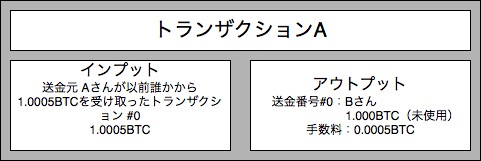
\includegraphics[width=80mm]{figures/txex1.jpg}
 \caption{トランザクションの例}
 \label{txex}
\end{figure}

作成されたトランザクションのアウトプットは、未だ相手が別のトランザクションのインプットしてい使用していないはずのアウトプットなのでこれは未使用のアウトプット、UTXOとなる。手数料とはこのトランザクションを検証しマイニングを行なったユーザに払われる報酬であり、マイニングの計算を行っているマイナーと呼ばれるユーザのモチベーションの1つとなっている。
\\
またトランザクションのインプット、アウトプットは1つのトランザクションに対して複数作られる場合がある。インプット、アウトプットが複数ある例を図\ref{txex2}に示す。

\begin{figure}[h]
 \centering
   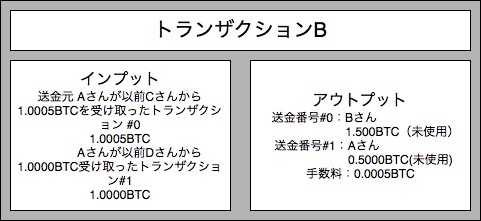
\includegraphics[width=80mm]{figures/txex2.jpg}
 \caption{複数のインプット、アウトプットを持つトランザクション}
 \label{txex2}
\end{figure}

送金したい額に対して、その額を超えるようなUTXOがなかった場合複数のUTXOを使用して送金を行う。図\ref{txex2}においては、送金したい額が1.5000BTCなのに対し、所持しているUTXOが1.0005BTCのものと1.0000BTCのものしかないためその2つを同時にインプットに使用している。またインプットして使用したUTXOの総額が相手に送金したい額よりも高かった場合、余剰分は自身に払い戻すため送金先を自分自身に設定してアウトプットを作成することになる。図\ref{txex2}ではインプットの総額が2.0005BTCなのに対し相手に送金したい額が1.500BTCなので、その差額からさらに手数料を引いた額を自分自身に送金している。\\
また、通常手数料は事前に金額を設定しているが、トランザクションにおいてはインプットの総額とアウトプットの総額として表現され明示的に表されることはない。

\subsection{ブロック}
ブロックチェーンにおいて1度に記録されるデータのまとまりをブロックと呼び、このブロックを時系列順に並べたものがブロックチェーンとなる。ビットコインにおけるブロックの構造を図\ref{block}に示す。

\begin{figure}[h]
 \centering
   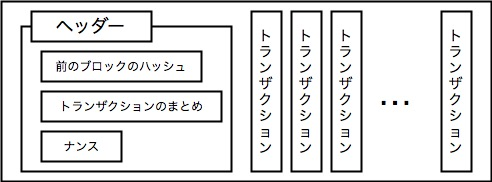
\includegraphics[width=80mm]{figures/blockdata.jpg}
 \caption{ビットコインにおけるブロックの構造}
 \label{block}
\end{figure}

ブロックは複数のトランザクションとヘッダからなり、またヘッダーは1つ前のブロックのハッシュ値、そのブロックに含まれるトランザクションのまとめ、ナンスからなる。\\
ナンスとはブロックのヘッダーからハッシュ値を求める際に与えるパラメータである。ビットコインにおいてブロックのハッシュ値は、事前に条件として設定された値以下にすることができなければブロックチェーンにブロックを記録できないようになっている。しかし、ヘッダーの中で前のブロックのハッシュとトランザクションのまとめはブロックが作られた時点で決まっており、この2つのみから求められるハッシュ値が条件を満たしているとは限らない。そこでナンスという自由に選択できるパラメータを設定し、ハッシュ値が条件を満たすように調整している。ハッシュ値の条件のことをDifficulty Targetと言い、条件と満たすようなナンスを1つ発見するまでに約10分の時間がかかるように調整されている。\\
またブロックチェーンでは、ブロックのハッシュ値を直後にブロックチェーンに記録されるブロックのヘッダーに含めることで過去のトランザクションの改竄を困難にしている。悪意あるユーザが過去のトランザクションを改竄しようとすると、そのトランザクションが含まれるブロックのヘッダーとハッシュ値が変わってしまい、各ブロックが一つ前のブロックのハッシュ値をヘッダーに所持していることとハッシュ関数の性質から、それ以降のブロックのヘッダーとハッシュ値も変わってしまう。ブロックチェーンでは最も繋がっているブロックが多く長さの長いチェーンを正当なチェーンとみなし、全てのユーザはそのチェーンにブロックを追加していくため、悪意あるユーザが改竄したデータを記録するためには改竄したブロック以降の全てのブロックにおいてハッシュ値を計算し直し、さらに他の全てのユーザが正当なチェーンを伸ばそうとする速度に勝たなくていけない。他の全てのユーザの計算能力の合計に勝利することが極めて難しいことからブロックチェーンの改竄は困難だと言われている。
\\
そして、ブロックチェーンのヘッダに含まれる取引データのまとめとはブロックに含まれるトランザクションのハッシュ値から作られるマークルルートである。マークルルートとは、複数のデータのハッシュ値を足し合わせ、その値からさらにハッシュ値を求めていき、最終的にただ1つのハッシュ値にまとめたものを言う。この時、ハッシュ値を2つずつ足し合わせ、そこから求めたハッシュ値をさらに別のハッシュ値と足し合わせていくと木構造ができ、この木構造をマークル木と呼ぶ。

\begin{figure}[h]
 \centering
   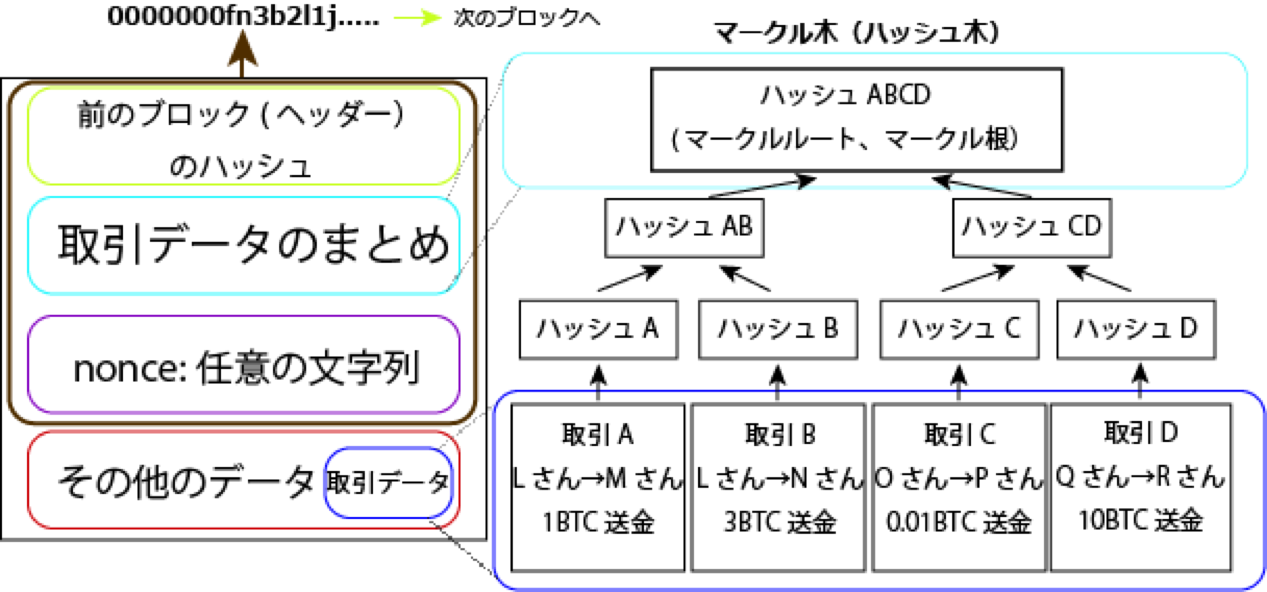
\includegraphics[width=80mm]{figures/markle.png}
 \caption{マークルルートとマークル木}
 \label{markle}
\end{figure}

このマークルルートを用いることでブロックに含まれるトランザクションが改竄されていないかの簡単な確認とSPVノードの実現が可能になった。マークルルートはブロックに含まれる全てのトランザクションの取引のまとめなので、そのどれか1つでもトランザクションが書き換えられればマークルルートも変化し、改竄を容易に検出できる。またマークルルートの存在によりユーザはブロックに含まれる全てのトランザクションの情報を持たなくてもブロックのヘッダーさえ持っていれば取引の検索が可能になった。SPVノードがある取引がブロックチェーンに記録されているか確認を行いたい時、ノードは付近のフルノードに確認したいトランザクション送信し問い合わせを行う。するとフルノードからトランザクションが含まれているブロックにおけるマークルルートといくつかのハッシュを受けとる。これは自信が確認したいトランザクションのハッシュ値と対となってマークルルートに至るためのハッシュ値となる。受け取ったハッシュ値と自身が確認したいトランザクションのハッシュ値からマークルルートを復元できれば、トラザクションがブロックに含まれていることが確認できる。\\
例として、あるSPVノードがトランザクションAを作成し、このトランザクションがブロックチェーンに記録されているか確かめる場合を考える。この時ユーザがフルノードから受け取るハッシュはハッシュB、ハッシュCD、マークルルートの3つである。ユーザは自身が最初から知っているハッシュAとハッシュBからハッシュABを計算でき、さらにハッシュABとハッシュCDからマークルルートを復元できる。この時ハッシュC、Dやブロックに含まれる他のトランザクションの情報は必要なく、たかだかマークル木の高さ分のハッシュ値だけでユーザはトランザクションがブロックチェーンに記録されているかを確認できる。

\begin{figure}[h]
 \centering
   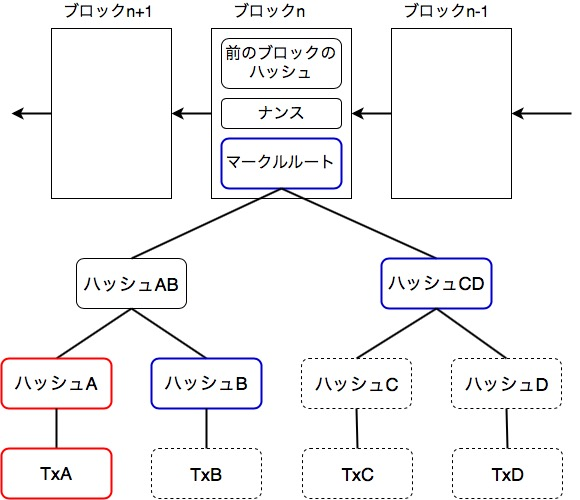
\includegraphics[width=80mm]{figures/marklepath.jpg}
 \caption{トランザクションAがブロックに含まれているか確認するために必要なハッシュ(赤線:ユーザが最初から持っている情報 青線:フルノードから受け取る情報)}
 \label{path}
\end{figure}

\subsection{マイニング}
ナンスの値はユーザが自由に設定できるが、ハッシュ関数の性質としてハッシュ値から入力を復号できない、つまりあるハッシュ値に対してどのような入力を与えればそのようなハッシュ値が求められるかわからないため、条件を満たすようなナンスの設定は総当たりで計算を行うのが一般的である。このナンスを求める作業をマイニングと呼ぶ。またマイニング作業を行うユーザのことをマイナーと呼ぶ。ビットコインにおけるマインングはProof of Work法(PoW法)と呼ばれる莫大な計算を行うことでブロックをブロックチェーンに追加する権利を得る方式である。

\begin{figure}[h]
 \centering
   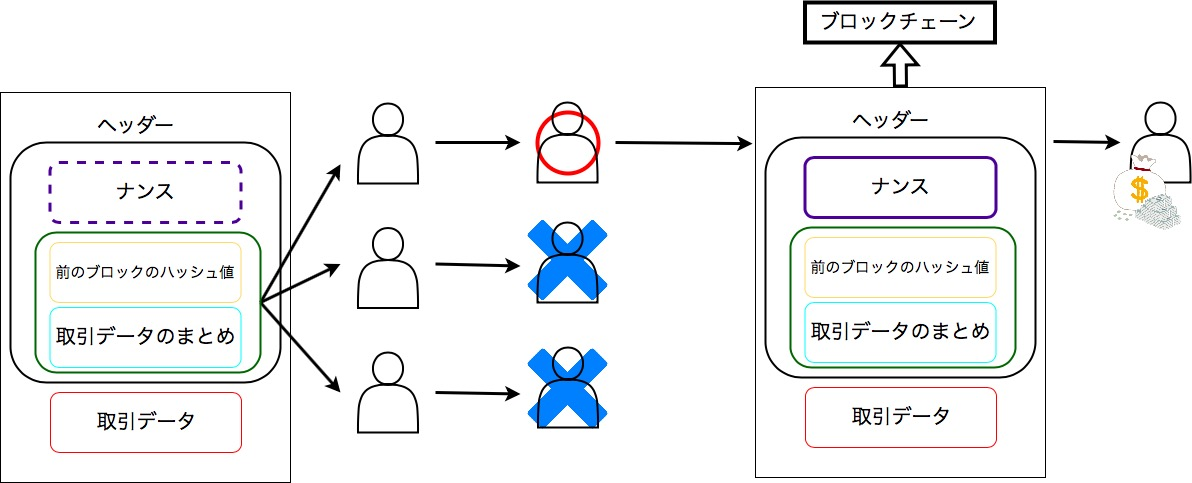
\includegraphics[width=100mm]{figures/PoW.jpg}
 \caption{ビットコインにおけるマイニングの流れ}
 \label{pow}
\end{figure}

PoWではナンスの計算が一番早かったユーザがブロックチェーンにブロックを追加する権利を得る。マイナーはいくつかのトランザクションを選択しブロックを作成する。そしてナンスの計算を行いブロックのハッシュ値がDifficulty Targetを満たすようなナンスを一番早く見つけることができたユーザがブロックチェーンにブロックを追加する。この時ブロックを追加できたユーザがブロックに含まれるトランザクションの手数料とブロックを追加したことに対する報酬としてコインベースと呼ばれる新しいビットコインを発行するトランザクションを得られる。この手数料とコインベースがマイナーがマイニングを行うインセンティブになっている。

\subsection{課題}
ブロックチェーンはビットコインなどの仮想通貨を始め様々な場所で活用され始めているが、まだいくつかの課題を残している。

\begin{itemize}
\item セキュリティ\\
ブロックチェーンに関する最近の研究においてビットコインに対する有効な攻撃方法が示されている\cite{security2}-\cite{security4}。これらの攻撃はブロックチェーンそのものではなく、ユーザ同士で構成されるネットワークやブロックチェーンのコンセンサスレイヤを利用することで敵対者の利益を大幅に高めている。
\item スケーラビリティ\\
ビットコインにおいて1秒間に処理できる取引数は7取引が限界だと言われている。これはマイニングの計算に1回10分程度の時間がかかるように難易度が決定されていること、1ブロックの最大容量が1MBとされているためである
。そのためビットコインでは2019年時点において常に10,000件~20,000件程度のトランザクションが未処理のまま処理されるのを待っている状態にある。さらにブロックチェーンを支払いのシステムとして見た場合、金融システムVisaにおける1秒間あたりの取引数約56,000トランザクションを処理する場合にも現在の秒間処理数では足りていない。このため現在のブロックチェーンの設計にはスケーラビリティに大きな問題があると言われている。

\end{itemize}

本研究ではこれらの課題の中でも特にスケーラビリティ問題に着目し、その解決策として提案されているマイクロペイメントチャネルとライトニングネットワークの拡張を目指す。

\section{スケーラビリティ問題の解決策}
\subsection{マイクロペイメントチャネル}
通常ビットコインでは取引が1回行われるたびにトランザクションを作成しブロックチェーンに記録していく。しかし、特定のユーザ同士が決まった合計金額内でお互いに送金し合う場合、周囲のユーザは残高の最終状態さえわかれば取引の途中経過には興味を示さないものと考えられる。マイクロペイメントチャネルとは特定の2者間における取引の開始と終了のみをブロックチェーンに記録することで、ブロックチェーンに記録しなくてはいけないトランザクション数の削減と送金に伴う手数料の増加を防ぐことでより少額での送金を可能にする。\\
マイクロペイメントチャネルを用いた送金の例を図\ref{chanel}~\ref{chanel3}に示す。

\begin{figure}[h]
 \centering
   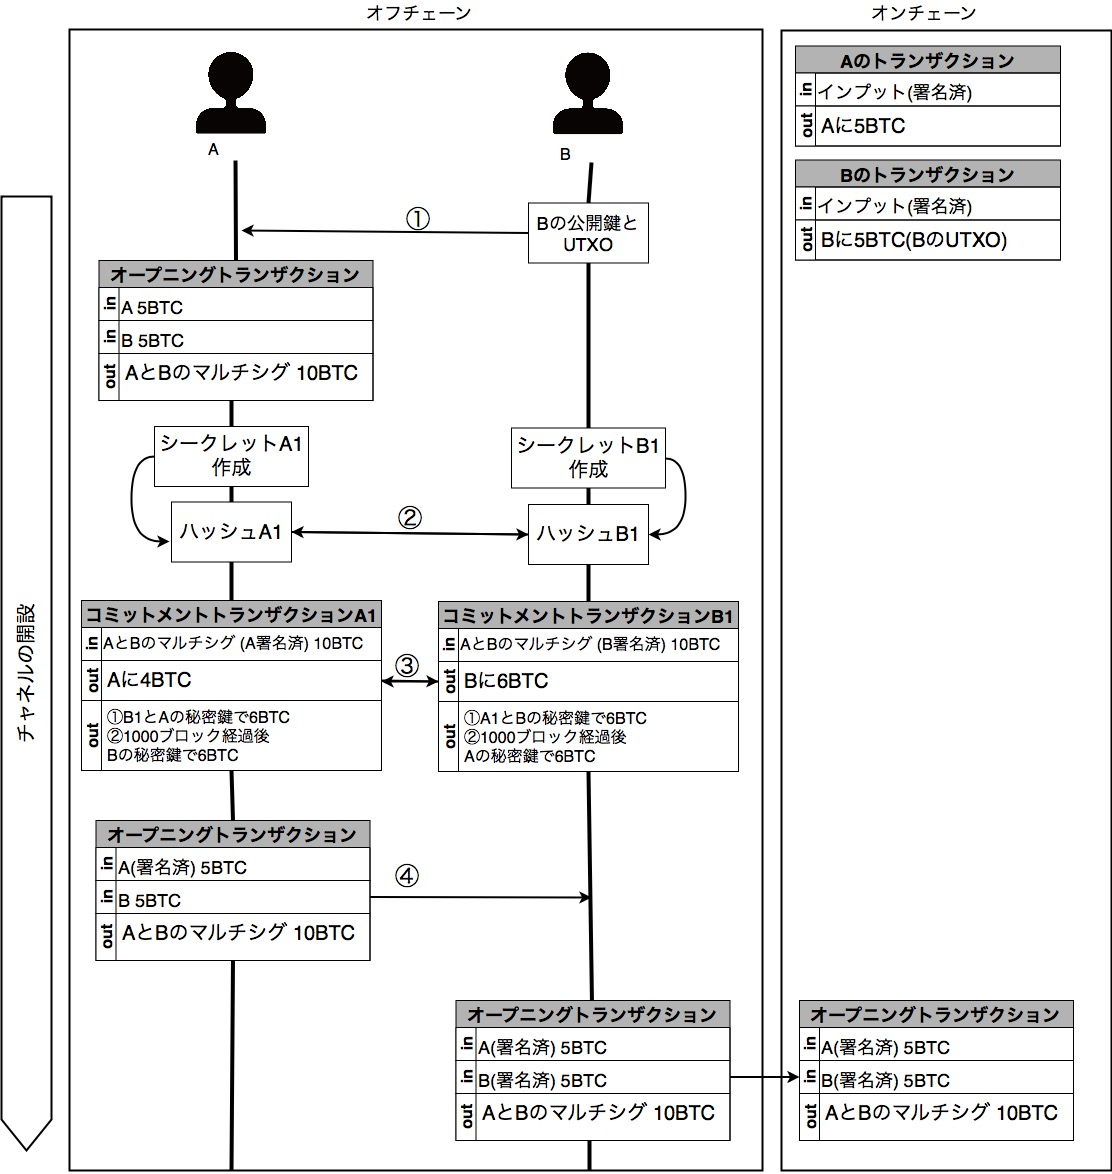
\includegraphics[width=100mm]{figures/maicrochanelpart1.jpg}
 \caption{マイクロペイメントチャネルの流れ-チャネルの開設}
 \label{chanel}
\end{figure}

\begin{itemize}
\item チャネルの開設
\begin{description}
\item[1] オープニングトランザシクションの作成\\
ユーザAはユーザBの公開鍵とチャネルの開設に使用するUTXOを受け取る。そして自身のUTXOとユーザBのUTXOをインプットに設定しオープニングトランザクションを作成する(ただしこの時点ではまだブロードキャストしない)。
\item[2] シークレットの作成とハッシュの交換\\
各ユーザはそれぞれ作成者しか知り得ないシークレットを作成する(このシークレットは後ほど相手と交換するので秘密鍵とは別に新しく作成する)。そのシークレットをハッシュ関数に入力することでシークレットのハッシュ値を計算する。そしてハッシュ値を相手と交換する。この時作成したシークレットは各ユーザがそれぞれ保管しておく(これによって相手が不正なトランザクションをブロックチェーンにブロードキャストすることを防ぐことができる)。
\item[3] コミットメントトランザシクションの作成、交換\\
ハッシュを交換したら、各ユーザはそれぞれ受け取ったハッシュを用いてコミットメントトランザクションを作成する。インプットにはオープニングトランザクションのアウトプットを使用する。アウトプットは作成するユーザによって異なる。\\
Aが作成するアウトプットは自身宛にお金を振り込むアウトプットと受けとったハッシュを用いて特別なスクリプトでロックしたアウトプットを使用する。Aのスクリプトによってロックされたアウトプットは以下のいずれかで使用できるようになる。
\begin{itemize}
\item 一定期間経過後Bの秘密鍵で入手できる
\item Bから受け取ったハッシュの元となるシークレットとAの秘密鍵で入手できる(このトランザクションを作った時点ではAはBのシークレットを知らないので入手できない)
\end{itemize}
Bが作成するコミットメントトランザクションはインプットは同じだがアウトプットが異なっている。Bが作成するトランザクションのアウトプットはBにお金を振り込むアウトプットとAから受け取ったハッシュを用いて特別なスクリプトでロックをかけたアウトプットとなる。このアウトプットは以下のいずれかで使用できるようになる。
\begin{itemize}
\item 一定期間経過後Aの秘密鍵で入手できる
\item Aから受け取ったハッシュの元となるシークレットとBの秘密鍵で入手できる(このトランザクションを作った時点ではBはAのシークレットを知らないので入手できない)
\end{itemize}
お互いにトランザクションを作成できたら、インプットに自分の署名を加え相手に送信する。受け取ったトランザクションは自分がインプットに署名し自分と相手双方の署名からなるマルチシグを完成させればいつでもブロードキャストすることができる。つまり自分が取引をブロックチェーンにブロードキャストしたい場合、ブロードキャストできるのは相手が作成したトランザクションとなる。

\item[4] オープニングトランザクションのブロードキャスト\\
オープニングトランザクションはどちらが作成しても構わない。片方がオープニングトランザクションに署名したならば、それを相手に送信し、受け取った側は自分も署名を行いブロックチェーンにブロードキャストする。この時点でチャネルが開設されたことがブロックチェーンに記録される。
\end{description}
\end{itemize}

\begin{figure}[h]
 \centering
   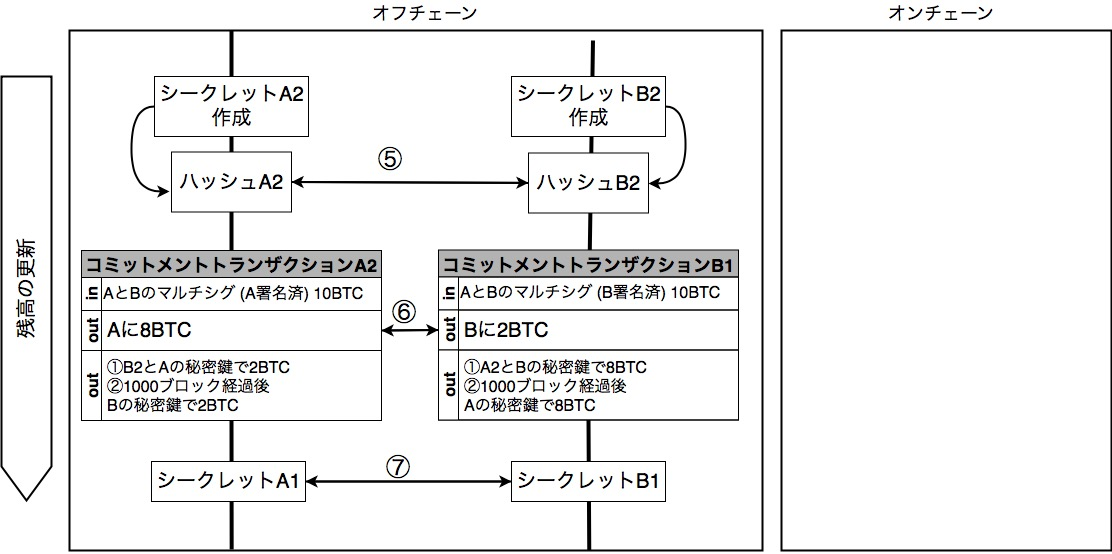
\includegraphics[width=100mm]{figures/maicrochanelpart2.jpg}
 \caption{マイクロペイメントチャネルの流れ-残高の更新}
 \label{chanel2}
\end{figure}

\begin{itemize}
\item 残高の更新\\
\begin{description}
\item[5] シークレットの作成と交換\\
チャネルの開設の手順2と同じようにそれぞれシークレットの作成とハッシュの計算、交換を行う。この時作成するシークレットはチャネルの開設で使ったものとは別のものにする必要がある。

\item[6] コミットメントトランザクションの作成、交換\\
チャネルの開設と同じようにコミットメントトランザクションを作成する。各ユーザへの資金の振り分けだけが変更されている。
\item[7] シークレットの交換\\
各ユーザは1つ前のコミットメントトランザクションを作成する際に使用したシークレットを交換する。これによって相手が古いコミットメントトランザクションをブロードキャストすることによって不当な利益を得ることを防げる。例えば、図\ref{chanel2}においてコミットメントトランザクションA2、B2を作成、交換し、シークレットA1、B1の交換も済ませた状態でユーザBが1つ前のコミットメントトランザクションA1をブロードキャストしたとする。トランザクションA1のアウトプットよりユーザAが4BTC即座に入手することができ、残りの6BTCは特別なスクリプトでロックがかかっている。このロックに関してBはシークレットB1は知っているがAの秘密鍵を知らないので一定期間経過するまで入手することができない。一方AはシークレットB1を交換してもらっているのでBがコミットメントトランザクションA1をブロードキャストした時点で即座に残り6BTCも入手することができる。結果としてユーザBはユーザAに全ての資金を取られてしまうため古いコミットメントトランザクションをブロードキャストして利益を得ることができなくなり、最新のコミットメントトランザクションだけがブロードキャストされるようになる。
\end{description}
\end{itemize}

\begin{figure}[h]
 \centering
   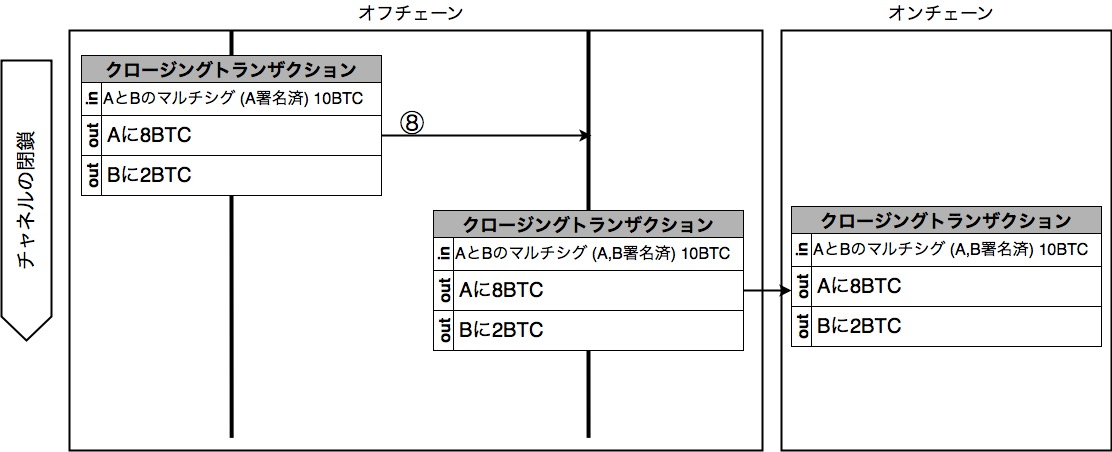
\includegraphics[width=100mm]{figures/maicrochanelpart3.jpg}
 \caption{マイクロペイメントチャネルの流れ-チャネルの閉鎖}
 \label{chanel3}
\end{figure}

\begin{itemize}
\item チャネルの閉鎖
\begin{description}
\item[8] クロージングトランザクションの作成とブロードキャスト\par
チャネルに参加しているユーザが最終的な残高の状態に合意し、チャネルを閉鎖することに合意したらクロージングトランザクションを作成する。まずユーザAもしくはユーザBがオープニングトランザクションのアウトプットをインプットとし、アウトプットは最新のコミットメントトランザクションにおける残高状態の通りに資金を振り分けるようにクロージングトランザクションを作成する。そしてユーザがお互いに署名を行いブロードキャストすることでチャネルを閉鎖できる。この時、ユーザ同士で意見の合意が得られない場合、クロージングトランザクションではなく最新のコミットメントトランザクションをブロードキャストすることでチャネルを強制的にクローズできる。
\end{description}
\end{itemize}

図\ref{chanel}より、ブロックチェーンに記録されるトランザクションはチャネル1つにつきせいぜい2つまでであるとわかる。これはチャネルの中でどれだけ残高の更新を行っても一定であり、取引の途中経過を記録しなくて良くなることからブロックチェーンに記録しなくてはいけないトランザクションの数を削減できる。\\
さらに、ブロックチェーンではトランザクションを作成し記録するたびにマイナーに手数料を支払わないといけない。この手数料は最低金額が決まっており、少額の取引は手数料が嵩むため行えなかった。しかし、マイクロペイメントチャネルでは途中の細かい取引はブロックチェーンに記録しないため手数料が発生せずこれまで以上に少額な取引が可能になった。

\subsection{ライトニングネットワーク}
マイクロペイメントチャネルはチャネルで繋がっているユーザ間で高速かつ安価な送金を可能にした。しかし、マイクロペイメントチャネルはチャネルで繋がっているユーザ間でしか送金を行うことができないという課題があった。チャネルを開く際にはブロックチェーンにオープニングトランザクションをブロードキャストする必要があり、大量にチャネルを開設することはスケーラビリティ、および手数料の面から好ましくない。ライトニングネットワークとはこれをチャネルで直接繋がっていないユーザ同士であっても送金を行えるように拡張したものである。
\par
ライトニングネットワークとはユーザをノード、ユーザ間で開設されているチャネルをエッジとするネットワークである。チャネルで繋がっていないユーザ間で送金を行う際には、送金者から受信者までのパスをネットワーク上で探索し、パス上にいるユーザを中継して送金を行う。このため送金者と受信者の間に直接チャネルが開いていなくても送金者、受信者がチャネルを開いている別のユーザを経由して送金を行うことができる。

\begin{figure}[h]
 \centering
   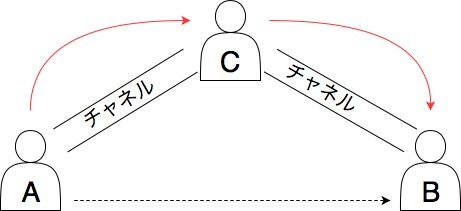
\includegraphics[width=100mm]{figures/multichanel2.jpg}
 \caption{チャネルで繋がっていないユーザ同士でも、間に別のユーザを中継することで送金を行える}
 \label{light1}
\end{figure}

間に取引と直接関係のない第3者を挟んで送金を行うとき、中継する第3者が資金を持ち逃げしないかを考慮しなくてはいけない。例えば図\ref{light1}ではユーザAからユーザBへの送金においてユーザCが中継を行なっている。この時ユーザAはまずユーザCに資金を送金し、それを確認したユーザCが同額をユーザBへと送金する。しかし、もしユーザCが資金を持ち逃げしようとした場合従来のマイクロペイメントチャネルの仕組みでは防ぐことができない。そこでライトニングネットワークは、間に第3者を挟んでも安全に送金を行うための仕組みとしてHashed TimeLock Contract(HTLC)を用いる。HTLCとはコミットメントトランザクションを作成する際に最終的な受信者が作成したシークレットハッシュを用いてアウトプットにロックをかけ、シークレットハッシュの元になったシークレットを提示するか一定時間経過しないと送金を受け取れないようにしたものである。HTLCを用いた支払いの例を図\ref{htlc}に示す。ユーザAからユーザCを中継してユーザBへと1BTCの送金が行われる。AC間、CB間にはチャネルが存在するがAB間には存在しない。ただし、チャネルが存在しないAB間でもハッシュやトランザクションの情報をやり取りすることはできる。

\begin{figure}[h]
 \centering
   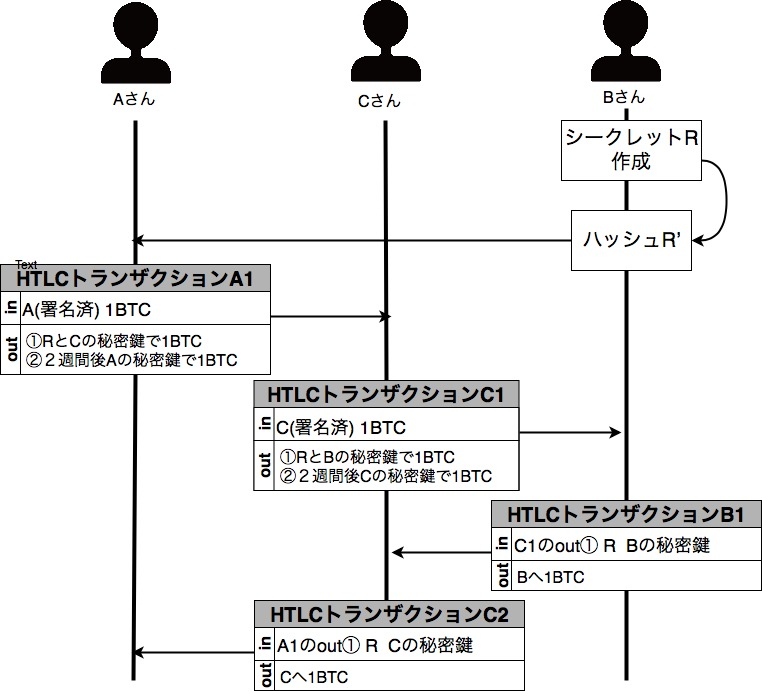
\includegraphics[width=100mm]{figures/HTLC.jpg}
 \caption{HTLCを用いた支払い}
 \label{htlc}
\end{figure}

\begin{itemize}
\item シークレットハッシュの作成、送信\\
最終的に資金を受け取るユーザBがシークレットRを作成し、シークレットハッシュを計算する。計算したシークレットハッシュをユーザA,Cに送信する。

\item ユーザAからユーザCへのHTLCトランザクションの作成\\
送金を開始するユーザAはBのシークレットのハッシュR'を受け取ったらHTLCトランザクションA1を作成する。インプットはAが送金する1BTC、アウトプットは以下の2つのどちらかで1BTCを入手できる。
\begin{itemize}
\item シークレットRとユーザCの秘密鍵
\item 2週間後Aの秘密鍵
\end{itemize}
1つ目のアウトプットはユーザBが資金を受け取った場合のみユーザCが知ることのできるシークレットRを用いてユーザCが資金を受け取るためのアウトプットである。シークレットRを用いることで中継するユーザはそのユーザの支払いが完了するまで資金を受け取れなくなっている。また2つ目のアウトプットはユーザCがユーザBへの支払いを行わず、いつまでもシークレットを提示できいまま2週間経過したときユーザAが資金を回収するためのアウトプットである。これにより中継するユーザが時間をかけてシークレットを割り出し資金を持ち逃げすることを防いでいる。作成したトランザクションはユーザCに送信する。

\item ユーザCからユーザBへのHTLCトランザクションの作成
ユーザAからHTLCトランザクションA1を受け取ったユーザCは同様にHTLCトランザクションC1を作成する。インプットはユーザBへと渡す1BTC、アウトプットは以下の2つどちらかで1BTCを入手できる。
\begin{itemize}
\item シークレットRとユーザBの秘密鍵
\item 2週間後Cの秘密鍵
\end{itemize}
作成したトランザクションC1をユーザBに送信する。

\item ユーザBが資金を受け取るトランザクションの作成。\\
トランザクションC1を受け取ったユーザBは、シークレットRを知っているので自身の秘密鍵で資金を受け取ることができる。資金を受け取るためのトランザクションがHTLCトランザクションB1である。C1のアウトプット1と自身の秘密鍵、シークレットをインプットとし1BTCを受け取っている。このトランザクションB1をブロードキャストすることでユーザA、CはシークレットRを知ることができる。

\item ユーザCが資金を受け取るトランザクションの作成。\\
トランザクションB1がブロードキャストされたことでユーザCはシークレットRを知ることができる。B1と同様にトランザクションC2をブロードキャストすることでユーザAからの資金を受け取ることができる。
\end{itemize}


\section{ライトニングネットワークのルーティング}
ライトニングネットワークは、単一の支払いにおいてお互いが直接には信頼していないユーザを経由して支払いを行うことができる。つまり、支払いを完了するために送金者と受信者との間に新しいチャネルを作成しなくても支払いを完了できる場合がある。そのためにライトニングネットワークにとって特に重要な問題が支払いルートのルーティングである。
\par
本節では現在提案されているいくつかのルーティングを説明する。中でもPavelらによって提案されたハイブリッドルーティングアルゴリズム「Flare」\cite{flare}について説明する。

\subsection{ルーティングアルゴリズムの概要}
\subsubsection{事前のアイデア} \label{sec:idea}
ライトニングネットワークのルーティングについて、ビットコインコミュニティはいくつかのアイデアを提案している。
\begin{description}
\item[ハブアンドスポークネットワーク]\leavevmode \\ 
ビットコインコミュニティが提案した初期のアイデア\cite{idea1}の1つはノードをウォレットノードとルーティングノードの2つのクラスに分類する方法である。前者のノードは支払いのみ、後者のノードは支払いのルーティング及び取引手数料の獲得のみが可能なノードとなる。この方法は全てのハブの情報によって任意のノードへのパスを発見できるため効率的にパスを発見することができる。一方で、この方法は一部のハブに支払いのルーティングが集中する可能性がある。またウォレットノードは支払いを行う以外のことができないのでオンライン状態を維持するインセンティブが存在しない。例えば支払いが受信者に一番近いハブで止まってしまい、ハブは受信者がオンラインになるまでオンライン状態を維持して待機しなくてはいけなくなる場合がある。この方法のもう1つの欠点は、フォールトトレランスである。ネットワーク状にハブが少数しかなく、そのうちの1つが停止した場合、ネットワーク全体が機能しなくなる可能性が存在する。
\\

\item[グローバルビーコン] \leavevmode \\
もう1つのアイデア\cite{idea2}はいくつかのノードをグローバルビーコンとしてランダムに選択し、特定の期間でビーコンセットを更新する方法である。全てのノードはビーコンへのパスを発見し、ビーコンを経由することで支払いを行う。この方法はネットワークが一部の少数グループによって制御されないという点でハブアンドスポークネットワーク方式より優れている。ただし、この方法はビーコンに選択されたノードの収益が非常に高くなるため自身がビーコンになるために偽のノードを作成される可能性がある。またビーコンの情報は公開されるので、ビーコンに選択されたノードはDoS攻撃の標的にされるリスクが存在する。加えて、グローバルビーコンにはネットワーク帯域幅、計算能力、及びチャネルに格納されている支払い能力が必要とされ、それらの条件を満たすノードは実際には非常に制限されるはずである。最後に、ビーコンに選択されたノードは選択されている間非常に多くのチャネルを作成する必要があるが、その多くは他のビーコンが選択された場合不要になる可能性がある。

\item[ローカルビーコン]\leavevmode \\
グローバルビーコンの発展として各ノードが個人ビーコンのリストをもつ方法が提案された\cite{idea3}。各ノードが独自に発見したビーコンのことをローカルビーコンという。支払いが送信されると送信者と受信者がビーコンリストを比較して支払いを行える交差点があるかを確認する。ローカルビーコンを用いるとネットワーク上のルーティングをグローバルビーコンより分散することができる。さらにこの方法は全てのノードが他のノードのビーコンに選択される可能性があるため、グローバルビーコンより取引手数料を均等に分配できる。これによりノードがオンライン状態を維持するインセンティブが生じ、ネットワークのルーティング機能が全体として向上するとされている。
\end{description}

\subsubsection{ハイブリッドアルゴリズム}
ライトニングネットワークは現在も開発が行われており、今後開発されるであろう構造や動作を推定してアルゴリズムを作成することは難しい。ただし、特定の側面ではライトニングネットワークはモバイルアドホックネットワーク(MANET)に似ている可能性がある。ライトニングネットワークとMANETには以下の類似点がある。
\begin{itemize}
\item ノード間のチャネルが頻繁に現れたり消えたりする。またチャネルの利用可能な容量が頻繁に変化するため特定のチャネルを介して支払いを送信することができない。
\item 新しいノードがネットワークに参加する、あるいは既存のノードがオフラインになることがある。
\item ネットワークの情報を自分で構成する必要がある。
\end{itemize}

ライトニングネットワークとMANETの類推は完全ではないが、ライトニングネットワークのルーティングはMANETにデプロイされたルーティングアルゴリズムのアイデアをいくつか応用することができる。MANETのルーティングアルゴリズムはプロアクティブ、リアクティブ、ハイブリッドの3つに分類できる\cite{MANET}。

\begin{description}
\item[プロアクティブ] \leavevmode \\
ネットワーク内のすべてのノードに関する最新のルーティング情報をルーティングテーブルの形式で保持する。この方法は大規模ネットワークにはスケーラブルでない。

\item[リアクティブ] \leavevmode \\
パス検索プロセスを作成し、パスが必要になった場合のみルーティングの情報を交換する方法。プロアクティブ型よりメモリ使用量に関して要求される量が少なくなる。

\item[ハイブリッド] \leavevmode \\
プロアクティブなルーティングとリアクティブなルーティングはトレードオフの関係にある。前者はレイテンシと信頼性の面で優れているが大規模なネットワークに対してスケーラブルでない。後者はスケーラブルではあるが、信頼性を犠牲にしている。ハイブリッドルーティングプロトコルは信頼性とスケーラビリティのバランスをとろうとする新しい方法である。
各ノードはネットワークのローカル部分のルーティングテーブルとアドレス距離の観点から送信者に近い遠隔ノードへのルートを保持する。ルーティング段階ではノードは中間ノードからパスの欠落部分を要求し、受信者へのパスを発見する。
\end{description}




ハイブリッドルーティングアルゴリズムFlareはMANETのハイブリッドルーティングプロトコルと同様にブロアクティブ及びリアクティブステージで構成されるアルゴリズムである。Flareにおけるプロアクティブ部分、リアクティブ部分\cite{flare}は以下のような働きをする。

\begin{description}
\item[ルート発見(プロアクティブ)] \leavevmode \\
Flareのプロアクティブ部分はノードの近隣の情報に基づくルーティングテーブルの構築とビーコンの選択になる。各ノードはルーティングテーブルの形でネットワークのローカル部分の知識を更新する。ルーティングテーブルはネットワークに存在することがわかっているチャネルの特定のサブセットである。ルーティングテーブルは受信者へのパスを発見することを目的に構築され、それが不可能な場合にはパスを見つけるのに役立つビーコンノードを決定する。
ビーコンは送信者のローカル部分を超えてランダムにノードを組み込むことでネットワーク全体のノードの可視性を強化できる。その結果、ノードはネットワークの完全な情報を持たなくても自身のルーティングテーブルとランダムに遠隔地に存在するビーコンの情報を合わせることで他のすべてのノードへ高い確率でパスを発見できるようになる。

\item[ルート選択(リアクティブ)] \leavevmode \\
Flareのリアクティブ部分はルーティングテーブルを利用したルート探索とそのランキング付けになる。ライトニングネットワークを介して支払いを送信することが決定されると、送信者は受信者への支払い可能なパスを見つける。送信者、受信者の2つのルーティングテーブルだけでパスを見つけることができなければ、受信者のビーコン及び他のノードのルーティングテーブルも使用する。
発見されたルートは事前に定義されたコスト関数によってランク付けされる。ランク付けははネットワークの静的情報と動的情報に分かれて行われる。
静的情報とは短時間の間に急速に変化することのないノード間の支払いチャネルの有無を指す。動的情報は急速に変化することのあるノードのステータスや支払いチャネル内の資金分配、チャネルの使用料を指す。
\end{description}

この2つのプロトコルを経てチャネルがランク付けされると、送信者は支払いに使用する最適なルートを選択する。実際にはルートのランク付けの段階で十分に評価値の高いルートが見つかれば、その時点でランキングを停止し、すぐに支払いを送信することもある。\\
また、フォールトトレランスの問題を回避するためリアクティブ部分では複数のパスが選択される必要がある。パス内の単一のノードが反応しなくなった場合には発見された別のパスを使用することで支払いを行うことができる。

\subsection{ライトニングネットワークのモデル}
ライトニングネットワークは$G=(V, E)$の無向グラフとして表される(図\ref{ln})。

\begin{figure}[h]
 \centering
   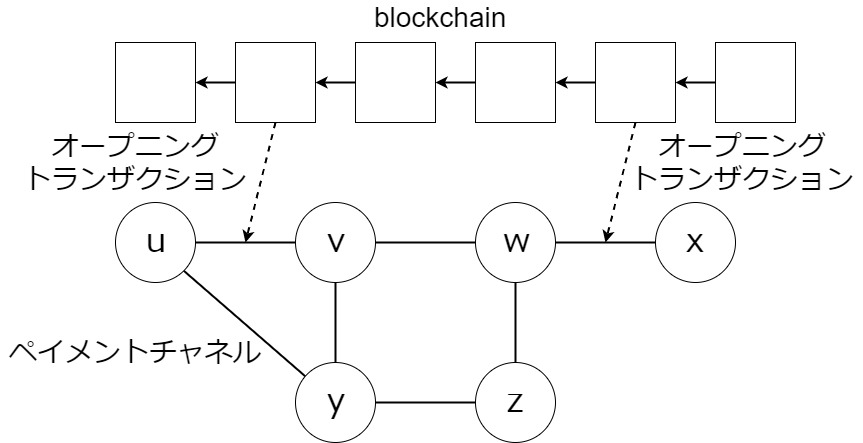
\includegraphics[width=100mm]{figures/LN.jpg}
 \caption{ライトニングネットワーク}
 \label{ln}
\end{figure}

$V$はネットワークに参加しているノードの集合で、$E \subseteq V^2$はノード間で開かれているチャネルの集合である。関数$Cap : V^2 \rightarrow [0, +\infty)$は、チャネル$e\in E$について、チャネルの容量$Cap(e)$を与える。チャネリの容量とは、オープニングトランザクションを作成するのに用いられたUTXOの金額の合計であり、チャネル内で一度に取引できる金額の上限となる。存在しないチャネルでは容量は0となる:
\begin{equation*}
\forall v_1,v_2\in V \ (v_1,v_2) \notin E \Leftrightarrow Cap(v_1,v_2) = 0.
\end{equation*}

さらに、ライトニングネットワークに関して、以下の5つを定義する。
\begin{itemize}
\item
任意の2ノード$x,y$間の\textbf{ホップ距離}$d_{node}(x, y)$は、ノードを接続するライトニングネットワークのチャネルの最少数である:
\begin{equation}
d_{node}(x, y) := \min \{ n\in \N : \exists v_1,\cdots,v_{n+1}\in V \ x=v_1,y=v_{n+1};\forall i\in 1,\cdots,n \ (v_i,v_{i+1}) \in E\}.
\end{equation}
\item
ノード$x\in V$とチャネル$e = (y,z)\in E$の\textbf{距離}はノード$x$とチャネルの両端間の距離の最小値である:
\begin{equation}
d_{chan}(x,(y,z)) := d_{chan}(x,e) := \min\{ d_{node}(x,y),d_{node}(x,z) \}.
\end{equation}
\item
ノード$v$と隣接しているノードの集合を$Adj(v)$として定義する:
\begin{equation}
\mbox{Adj}(v) := \{z\in V| d_{node}(v,z) = 1 \}.
\end{equation}
\item
チャネルの集合$T \subseteq E$に対し、$Nodes(T)$は$T$に含まれるチャネルによって接続されたノードの集合である:
\begin{equation}
\mbox{Nodes}(T) := \{a \in V | (a,\cdot) \in T \vee (\cdot, a) \in T \}.
\end{equation}
\item
各ノードは固有のIDキーを所持しており、IDキーのSHA-256\cite{sha256}として計算された256ビット整数をノードのアドレスとして定義する。またノード$x,y\in V$間の\textbf{アドレス距離}を$\rho(x,y)$を、ノードアドレスのビットのXOR演算の結果とする。
ノードアドレスはビーコンの選択に使用され、送信者とアドレス距離が近い点を選択することで、ネットワーク内のノードをランダムビーコンとして選択し、受信者へのパスを発見できる確率を高めることができる。
\end{itemize}

\subsection{ルーティングテーブル}
ルート検出のために各ノードはルーティングテーブルを構築する。ノード$v\in V$のルーティングテーブル$v.RT$は$v$との距離が近隣半径$r_{nb} \in \N$以下の場所に存在するすべてのチャネルのサブセットとなる
\begin{equation*}
v.RT := \{ (u,w)|d_{chan}(v,(u,w)) \leq r_{nb} \}.
\end{equation*}

またルーティングテーブルを構築するためにチャネルに関する情報を収集する過程でチャネルの総容量の情報も取得する。図\ref{ln}におけるノード$v$のルーティングテーブルに格納される情報は表\ref{rt_samp}のようになる
\\
\begin{table}[h]
\centering
\caption{ノード$v$のルーティングテーブルに含まれる情報}
\begin{tabular}{cc|c}
ノード1 & ノード2 & 容量 \\
\hline
u & v & 0.5BTC \\
v & y & 0.3BTC \\
v & w & 0.1BTC \\
u & y & 0.001BTC \\
y & z & 4BTC \\
w & z & 1BTC \\
\end{tabular}
\label{rt_samp}
\end{table}
\\
ルーティングテーブルを用いたルート検出の例を図\ref{rt}に示す。$r_{nb}$は2とする、

\begin{figure}[h]
 \centering
   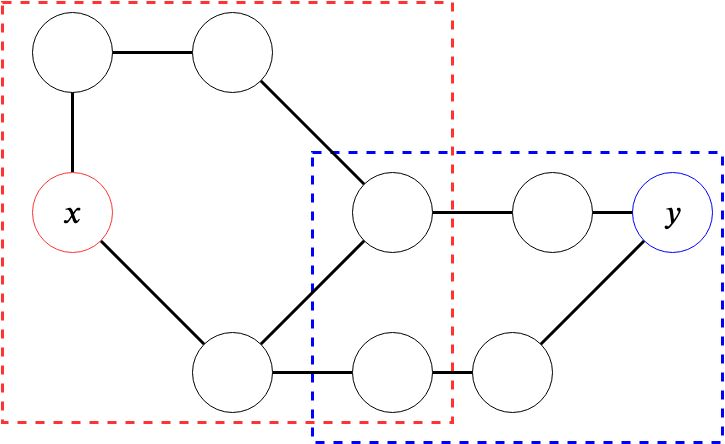
\includegraphics[width=100mm]{figures/RT.jpg}
 \caption{RTによるルート検出}
 \label{rt}
\end{figure}

送信者$x$は自身のRT,$x.RT$の中から受信者へのパスを探索し、見つからなければ受信者$y$へ$y.RT$を要求する。受け取った$y.RT$を自身を$x.RT$とマージし、その中で再び受信者へのパスを探索する。

\subsection{近隣の探索}
Flaraにおいて各ノードは自身の近隣の情報をRTとして保持している。しかし、ライトニングネットワークは動的に変化するネットワークであり現在のRTが今後も使用できるとは限らない。そのため各ノードは自身の近隣を探索しRTを更新していかなくてはいけない。\\
近隣を探索するメカニズムはメッセージNEIGHBOR\_HELLO,NEIGHBOR\_UPD,NEIGHBOR\_RST,\\REIGHBOR\_ACKに基づいて行われる。
\begin{itemize}
\item NEIGHBOR\_HELLOはメッセージの受信者の完全なRTを送信者に送信する。
\item NEIGHBOR\_UPDは、最後に送信された更新メッセージ以降に変更されたライトニングネットワークの変更をノードのRTに反映させる。
\item NEIGHBOR\_RSTは更新情報が失われたと思われる際に送信され、受信者の完全なRTを送信者に送信する。
\item NEIGHBOR\_ACKはNEIGHBOR\_HELLO,NEIGHBOR\_UPDへの応答として扱われ、ノードがメッセージを適切に処理したことを表す。
\end{itemize}

ノードは隣接ノードからのNEIGHBOR\_メッセージのみを受理する。新しくチャネルが追加されRTが更新される時のメッセージ送信のフローを図\ref{NBmes}に示す。

\begin{figure}[h]
 \centering
   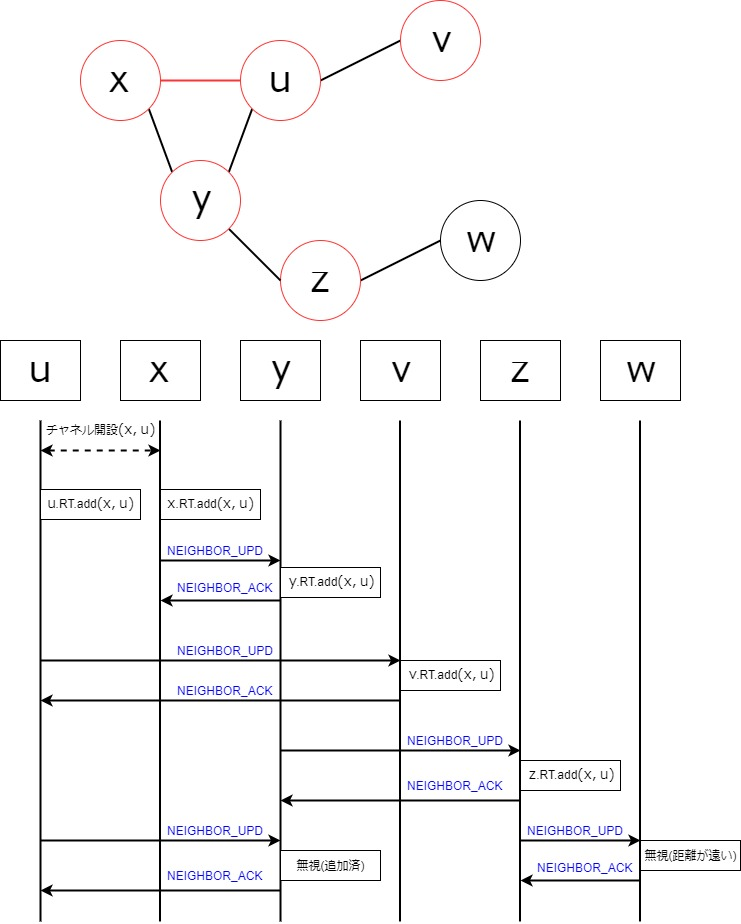
\includegraphics[width=100mm]{figures/NBmes.jpg}
 \caption{RT更新時のメッセージフロー}
 \label{NBmes}
\end{figure}

図\ref{NBmes}において、ノード$x,u$間に新しいチャネルが開設された場合を考える。近隣半径$r_{nb}$は2とする。ノード$x,u$は自身のRTに開設したチャネルを追加し、隣接しているノード$y,v$にNEIGHBOR\_UPDメッセージを送信する。NEIGHBOR\_UPDメッセージを受信したノード$y,v$は新しく解説されたチャネルと自身との距離$d_{chan}$を計算し、それが$r_{nb}$以下なら自身のRTに追加する(RT.add)。そして、送信者にNEIGHBOR\_UPDメッセージを処理したことを伝えるためにNEIGHBOR\_ACKメッセージを送信する。RTにチャネルを追加したノード$y,v$はさらに自身の隣接ノード$z$にNEIGHBOR\_UPDメッセージを送信する。$z$は新しく解説されたチャネルと自身との距離$d_{chan}$を計算し、それが$r_{nb}$以下なら自身のRTに追加し、NEIGHBOR\_ACKメッセージを$y$に送信する。そして、さらに自身の隣接ノード$w$にNEIGHBOR\_UPDメッセージを送信する。NEIGHBOR\_UPDメッセージを受信した$w$は$d_{chan}$を計算し、それが$r_{nb}$より大きいのでチャネルをRTに追加しない。NEIGHBOR\_UPDメッセージを処理したことを伝えるためにNEIGHBOR\_ACKメッセージは送信する(RTを更新していないので$w$はNEIGHBOR\_UPDメッセージを送信しない)。またノード$u$は隣接ノード$y$にもNEIGHBOR\_UPDメッセージを送信するが、この時$y$は既にチャネルをRTに追加しているのでRTを更新しない。
これらのメッセージを利用したノードのRT更新のアルゴリズムを以下に示す。

\begin{algorithm}
 \caption{近隣情報に基づくRTの更新}
 \begin{algorithmic}[1]
 \renewcommand{\algorithmicrequire}{\textbf{Input:}}
 \renewcommand{\algorithmicensure}{\textbf{Output:}}
 \REQUIRE 受信者$u$ \\
 送信者$v$ \\
 メッセージ内の新しく開かれたチャネルのセット$M \subset E$ \\
 メッセージ内の閉じたチャネルのセット$Mr \subset E$(NEIGHBOR\_HELLOの場合$Mr = \emptyset$) \\
 近隣半径$r_{nb} \geq 1$
 \ENSURE  更新された$u.RT$
 \\ \textit{Initialisation} :
  \STATE $u.RT$と新しく開かれたチャネルのセット$M$をマージ:$RT_{pre} = u.RT \cup M$
  \STATE $RT_{pre}$に基づくネットワーク$G = (Nodes(RT_{pre}), RT_{pre})$を作成
 \\ \textit{LOOP Process}
  \FOR {$e \in M \backslash u.RT $}
  \STATE $G_{pre}$におけるノード$u$とチャネル$e$の最小距離を計算:$d = d_{chan}(u,e)$.$G_{pre}$が連結でなく距離を計算できなければ$d = +\infty$とする
  \IF {($d \leq r_{nb}$)}
  \STATE $e$の容量$Cap(e)$を取得
  \STATE $u.RT = u.RT \cup \{e\}$.$Cap(e)$を保存
  \ENDIF
  \ENDFOR
  \FOR {$e \in Mr \cap u.RT$}
  \STATE ブロックチェーン上でチャネル$e$が閉じられているか確認
  \IF {チャネル$e$が閉じられていることが確認できた}
  \STATE $u.RT = u.RT \backslash {e}$ 
  \ENDIF
  \ENDFOR
 \end{algorithmic} 
 \end{algorithm}

\subsection{ビーコンの探索}
Flareにおいてビーコンはネットワーク上のランダムな遠方に存在するノードとして定義される。各ノードはビーコンを検出することにより、ビーコンの近隣を認識することで探索できるネットワークの範囲を拡大することができる。ノード$u \in V$のビーコンは$u.bc$と表され、アドレス空間でノード$u$に最も近いノードを選択する。
\begin{equation*}
\forall v \in u.bc, \forall z \in V \backslash (\{u \} \cup u.bc) \ \rho(v,u) < \rho(z,u).
\end{equation*}

実際にはビーコンの検出も各ノードのRTと、近隣のノードのRT内で行われるため、すべてのノードの中からアドレス空間においてノード$u$に最も近いノードが選択されるとは限らないが、これはビーコンの役割には影響しない。
\\
ビーコンの検出はBEACON\_REQ,BEACON\_ACK,BEACON\_SETメッセージに基づいて行われる。
\begin{itemize}
\item BEACON\_REQはビーコン候補となることをノードに通知するために送信される。
\item BEACON\_ACKはBEACON\_REQへの応答として送信され、ノードがビーコン候補になることに同意する。また、自身の近隣により良いビーコン候補があるかどうかを確認する。もしより良いビーコン候補があるなら、そのノードとノードへのパスを一緒に送信する。例えば、ノード$u$からノード$v$へBEACON\_REQメッセージが送信される場合、BEACON\_ACKメッセージとして$v$よりアドレス空間で$u$に近いノードの集合$Cv=\{z \in Node)(v.RT)| \rho(z,u) < \rho(v,u)\}$と$v$から$z\in Cv$へのパス$Mv$を送信する。もし自身より良いビーコン候補がなければ$Cv,Mv$は空になる。
\item BEACON\_SETはノードがビーコンとして選択されたことを通知するために送信される。
\end{itemize}

ビーコンを見つけるために、ノードは自身のRTからアドレス空間で自身に一番近いノードにBEACON\_REQメッセージを送信する。メッセージを受け取ったノードは自身のRT内でより良いビーコン候補があるかを探索し、その結果をBEACON\_ACKメッセージとして送信者に通知する。送信者はBEACON\_ACKで新しく見つかったノードをビーコン候補に追加し、同様のビーコン探索プロセスを繰り返す(図\ref{rtbc})。最後にノードはビーコン候補の中から自身のビーコンを$N_{bc}$個選択する(\textbf{Algorithm2})。

\begin{figure}[h]
 \centering
   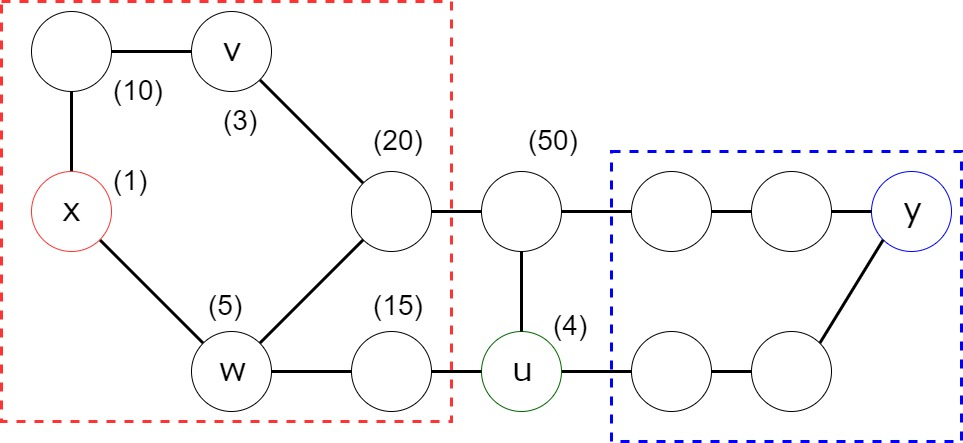
\includegraphics[width=100mm]{figures/RTBC.jpg}
 \caption{ビーコン検出}
 \label{rtbc}
\end{figure}

\begin{algorithm}
 \caption{ビーコンの探索}
 \begin{algorithmic}[1]
 \renewcommand{\algorithmicrequire}{\textbf{Input:}}
 \renewcommand{\algorithmicensure}{\textbf{Output:}}
 \REQUIRE 受信者$u$ \\
 ビーコンの数$N_{bc} > 0$
 \ENSURE  更新された$u.bc$
 \\ \textit{Initialisation} :
  \STATE ビーコン候補ノードの集合の初期化:$B = Nodes(u.RT)$
  \STATE 探索済みノード集合の初期化:$U = \emptyset$
  \STATE メッセージ受理済みノード集合の初期化:$R = \emptyset$
 \\ \textit{LOOP Process}
  \WHILE {$|B| > 0$}
  \STATE 未処理のビーコン候補$v$を一つ選択する:$v := \argmin_{z\in B} \rho(z,u)$
  \STATE $v$を処理済みとして記録:$U = U \cup {v}; \ B = B \backslash {v}$
  \STATE $v$にBEACON\_REQメッセージを送信。BEACON\_ACKメッセージが返ってくるのを待つ
  \IF {BEACON\_ACKがタイムアウト}
  \STATE 次のノードで探索を続ける
  \ENDIF
  \STATE BEACON\_ACKが$Cv,Mv$を返してきたと仮定する。
  \STATE $v$を受理済みとして記録:$R = R\cup {v}$
  \FOR {$z \in Cv \backslash (B \cup U)$}
  \STATE $\rho(z,u) < \rho(v,u)$を確認
  \STATE $Mv(z)$が$v$から$z$へのパスになっているかを確認
  \STATE $Mv(z)$に含まれているチャネルがブロックチェーン上で閉じていないか確認
  \STATE $z$をビーコン候補に追加:$B = B\cup {z}$
  \ENDFOR
  \WHILE {$|B| > N_{bc}$}
  \STATE ビーコン候補から、ホップ距離が$u$に近いノードを削除する
  \STATE $z^* = \argmin_{z \in B} d_{node}(u,z); \ B = B \backslash {z^*}$
  \ENDWHILE 
  \ENDWHILE
  \FOR {$v \in R $,$R$はアドレス距離順にソートしておく}
  \STATE $v$からBEACON\_SETメッセージを送信し$u$のビーコンとする:$u.RT = u.RT \cup {v}$
  \STATE $v$へのパスを$u.RT$に追加
  \IF {$|u.bc| = N_{bc}$}
  \STATE exit 
  \ENDIF
  \ENDFOR
 \end{algorithmic} 
 \end{algorithm}

\subsection{ルート選択}
Flareではルーティングアルゴリズムにおけるルート選択を大きく2つの部分に分類している。
\begin{description}
\item[静的ランキング] 送信者はRTの情報を利用して送金ルートの候補を選択する。これを実行するために送信者は受信者とアドレス空間で受信者に近いノードにRTを要求する。受信したRTには受信者へのパスが含まれている可能性がある。送信者はRTの情報に基づいて受信者への最短経路のランキングを作成し、次の動的ランキングを行う。
\item[動的ランキング] 送信者から受信者への有効なパスが発見出来たら、そのパスに対してネットワークの動的な情報(急速に変化することのあるノードのステータスや支払いチャネル内の資金分配、チャネルの使用料)を用いてランキング付けを行う。このランキング付けは事前に何らかのコスト関数を定義して行う。
\end{description}

ルート選択では2種類のメッセージを使用する。
\begin{itemize}
\item TABEL\_REQは受信者にRTの完全な情報を要求する。
\item TABLE\_RESPはTABEL\_REQの応答として送信され、送信者の完全なRTを送信する。
\end{itemize}

上記の静的ランキングに対するアルゴリズムをアルゴリズム3に示す。まず初めに送信者のRTから受信者へのパスを探索する。次に受信者のRTを要求し、送信者のRTとマージして統合されたRTでルートを探索する。それ以降は送信者が既知のパスを持ち、アドレス距離が受信者に近いノードにRTを要求し、ルートを探索する。ルートの探索のために$paths(s, r, RT, k)$を定義する。$paths(s, r, RT, k)$はダイクストラ法とYenのアルゴリズム\cite{Yen}を用いて送信者から受信者へのルートを$k$本発見する。

\begin{algorithm}
 \caption{静的ランキング(候補ルートの探索)}
 \begin{algorithmic}[1]
 \renewcommand{\algorithmicrequire}{\textbf{Input:}}
 \renewcommand{\algorithmicensure}{\textbf{Output:}}
 \REQUIRE 送信者$u$ \\
 受信者$r$ \\
 発見するパスの最大数$k \geq 1$ \\
 メッセージを送信するノードの最大数$N_{tab} \geq 1$ 
 \ENSURE  発見された$s$から$r$へと至るルートの集合$P$($P = \emptyset$はルーティングが失敗したことを表す)
 \\ \textit{Initialisation} :
  \STATE 送信者のRTで探索に使うRTを初期化:$RT_{co} = s.RT$
  \STATE ルートの集合を初期化:$P = \emptyset$
  \STATE 送信者からTABLE\_REQメッセージを受け取ってRTを送信したノードの集合を初期化:$U = \emptyset$
 \\ \textit{LOOP Process}
  \WHILE {$|P| > k \wedge |U| < N_{tab}$}
  \STATE $RT_{co}$で送信者$s$から受信者$r$へのルートを$k$本まで探索する。
  \begin{equation*}
P = P \cup Paths(s, r, RT_{co}, k)
\end{equation*}
  \IF {$|P| < k$}
  \STATE $RT_{co}$に含まれているノードの中で受信者$r$にアドレス距離が最も近いノードを一つ選択する。
  \begin{equation*}
  c = \argmin_{z \in Nodes(RT_{co} \backslash U)} \rho(z, r)
  \end{equation*}
  \STATE TABLE\_REQメッセージを送信してノード$c$にRTを要求する。
  \begin{equation*}
  RT_{co} = RT_{co} \cup c.RT
  \end{equation*}
  \STATE $U = U \cup {c}$
  \ENDIF 
  \ENDWHILE
  \RETURN $P$ 
 \end{algorithmic} 
 \end{algorithm}
 
この時チャネルの総容量で$RT_{co}$をフィルター処理できる。チャネル$e$の総容量$Cap(e)$が送信者が送金しようとしている金額$f$よりも低い場合$RT_{co}$でルートを探索するときそのチャネルを無視することができる。ただし、支払いが複数のチャネルに分かれて行われる場合この処理は逆効果になる。

\subsection{候補ルートのランキング}
アルゴリズム3で候補ルートの集合$P$を作成した後、ネットワークの動的情報に基づいて発見したルートをランキング付けする。この処理はアルゴリズム3で新しいルート$p\in P$が発見されるたびに行われ、候補ルートの評価値$rr(p) \in [-\infty, +\infty)$を返す。またアルゴリズムの処理時間を短縮するために何らかの閾値$r_{good}$を定義しておき、評価値$rr(p)$が$r_{good}$を超えれば発見したルートの数が$k$本未満であっても、そのルート$p$を送金ルートとして決定しルーティングアルゴリズムを即座に終了することができる。
\\
評価値$rr(p)$は何らかの評価関数によって計算される。本稿ではこれを支払いに使用するすべてのチャネルの使用料の合計$C$を用いて
\begin{equation}
rr(p) = \frac{1}{C}
\end{equation}
とした。

\section{数値実験}

\subsection{実験環境}
実験に用いた環境は以下の通り。

\begin{table}[h]
	\begin{center}
    \caption{実験環境}
		\begin{tabular}{|c|c|c|c|}
			\hline
            OS & CPU & 言語 & メモリ\\
            \hline
            \shortstack{Mac OS Sierra \\ version.10.12.6} & \shortstack{3.2GHz \\intel core i5} & Python3.7.0 & \shortstack{8GB\\RAM} \\
            \hline
		\end{tabular}
        \label{track}
	\end{center}
\end{table}

\subsection{実験1}
\subsubsection{実験内容}
ハイブリッドルーティングアルゴリズム「Flare」を用いてライトニングネットワークにおけるルート探索を行った。ライトニングネットワークはノード数$|V|=1000$のスモールワールドネットワーク\cite{swn}として作成した。このとき、パラメーターとして
\begin{itemize}
\item スモールワールドネットワークの近隣の数:4
\item 再配線の確率:0.3
\item $r_{nb} = 2$
\item $k=10$
\end{itemize}
を与えた。\\
実験では$V$から送信者としてノード$n_{samp}$をランダムに10個選択し、$n_{samp}$から他のランダムに選ばれた100個のノードへのパスを探索した。この時、ビーコンの数$N_{bc}$とRTを要求するノードの数$Q$を変化させることでパスを見つけることができた割合がどう変化するのかを確認した。$N_{bc}=\{0,1,2,3,4,5,6,7,8,9,10,11\}$、$Q=\{0,1,10\}$として実験を行なった。

\subsubsection{実験結果}
パスを見つけることのできた割合をを表\ref{ans1t}と図\ref{ans1f}に示す。

\begin{table}[h]
	\begin{center}
    \caption{パスを見つけることのできた割合}
		\begin{tabular}{|c|ccc|}
			\hline
            $N_{bc}$ \textbackslash $Q$ & 0 & 1 & 10\\
            \hline
			0  & 0.03  & 0.357 & 0.963\\
			1  & 0.037 & 0.425 & 0.967\\
			2  & 0.057 & 0.525 & 0.973\\
			3  & 0.068 & 0.571 & 0.973\\
			4  & 0.079 & 0.626 & 0.977\\
			5  & 0.083 & 0.653 & 0.979\\
			6  & 0.093 & 0.713 & 0.982\\
			7  & 0.102 & 0.73  & 0.982\\
			8  & 0.107 & 0.746 & 0.981\\
			9  & 0.113 & 0.751 & 0.981\\
			10 & 0.124 & 0.781 & 0.983\\
			11 & 0.133 & 0.8   & 0.982\\
            \hline
		\end{tabular}
        \label{ans1t}
	\end{center}
\end{table}

\begin{figure}[h]
 \centering
   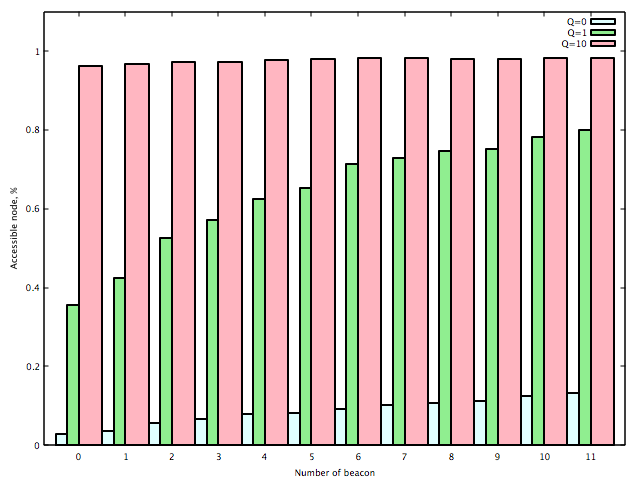
\includegraphics[width=100mm]{figures/ex1accessible.png}
 \caption{パスを見つけることのできた割合}
 \label{ans1f}
\end{figure}

また、この実験において計算にかかった時間は以下の通りであった。

\begin{figure}[h]
 \centering
   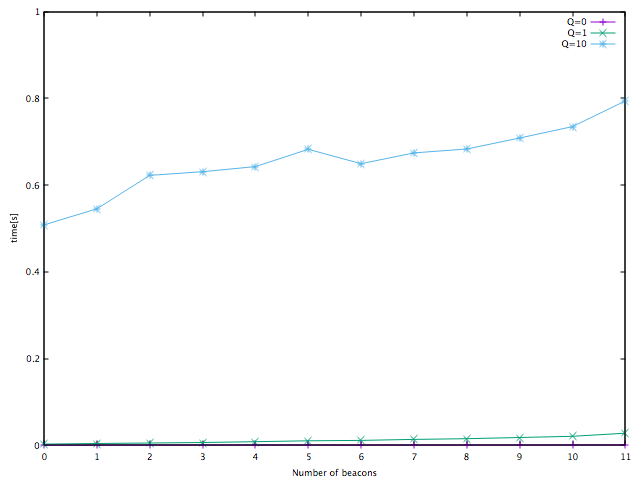
\includegraphics[width=100mm]{figures/avetime.png}
 \caption{計算時かかった時間}
 \label{time1}
\end{figure}

\subsection{実験2}
\subsubsection{実験内容}
実験1と同様のパラメータでノード数$|V|=2000$のライトニングネットワークを作成した。このライトニングネットワークにおいて、ランダムに送信者としてノード$n_{samp}$を10個選択し、$n_{samp}$から他のすべてのノードへのパスを探索した。この時、ビーコンの数$N_{bc}$とRTを要求するノードの数$Q$を変化させることでパスを見つけることができた割合がどう変化するのかを確認した。$N_{bc}=\{0,1,2,3,4,5,6,7,8,9,10,11\}$、$Q=\{0,1,10\}$として実験を行なった。

\subsubsection{実験結果}
実験結果を表\ref{ans2t}と図\ref{ans2f}に示す。

\begin{table}[h]
	\begin{center}
    \caption{$|V|=2000$でパスを見つけることのできた割合}
		\begin{tabular}{|c|ccc|}
			\hline
            $N_{bc}$ \textbackslash $Q$ & 0 & 1 & 10\\
            \hline
			0 & 0.0 & 0.01535 & 0.78405 \\
			1 & 0.0 & 0.0185 & 0.8155\\
			2 & 0.0 & 0.02285 & 0.84985\\
			3 & 0.0 & 0.02695 & 0.86765\\
			4 & 0.0 & 0.03045 & 0.87365\\
			5 & 0.0 & 0.0345 & 0.88075 \\
			6 & 0.0 & 0.0371 & 0.88575 \\
			7 & 0.0 & 0.03985 & 0.88995\\
			8 & 0.0 & 0.0439 & 0.89385 \\
			9 & 0.0 & 0.0474 & 0.89595 \\
			10 & 0.0 & 0.05085 & 0.8977\\
			11 & 0.0 & 0.05345 & 0.9011\\
            \hline
		\end{tabular}
        \label{ans1t}
	\end{center}
\end{table}

%%%
%ここに取り直したデータを入れる
%%%

また、この実験において送受信1組辺りの送金パスを発見するのにかかった平均時間を図\ref{time2}に示す。

%%%
%同上
%%%

\subsubsection{考察}
実験1、実験2を通してビーコンの数$N_{bc}$を増やすことでパスを発見できる確率が高くなっていることが確認できた。これはビーコンの数を増やすことでより送信者から遠方に存在するノードへRTを要求できる確率が高くなり、遠方に存在しているかもしれない受信者の近隣を認識しやすくなるからだと思われる。またRTを要求できるノードの数$Q$については、これも多くすればするほどパスが見つかりやすくなっている。これはより多くのノードにRTを要求できた方が送信者が認識できる範囲が広がり受信者を見つけやすくなるためだと考えられる。\\
パスを見つけるのに要する時間については、現時点で最も時間がかかっている$|V|~2000,Q=10$での探索でも1回あたり平均1.26秒ほどでパスが見つかっており、十分に現実的な時間でパスが探索できていると考える。

\subsection{実験3}
\subsubsection{実験内容}
ライトニングネットワークにおいてランダムに選択された送受信の組でパスを探索した時、必ず使用する、もしくは頻繁に使用するチャネルが存在していないか確認したい。\\
ノード数$|V|=2000$のライトニングネットワークを作成し、その中から送信者ノード$n_{samp}$を選択する。$n_{samp}$から他のランダムに選ばれた100個のノードへの送金パスを探索する。%この時、発見できたパスで使用しているチャネルを確認し、見つかったパスのうち何割のパスがそのチャネルを使用しているのか、最も使用されているチャネルは何割のパスで使用されているのかを確認する。
また特徴的な形状のネットワークとしてハブアンドスポーク型のライトニングネットワークの場合、頻繁に使用されるパスが存在するか、存在するなら最大でどれくらいの確率でパスが使用されるのか、通常のネットワークと特殊な形状のネットワークで、ネットワークの更新を行った際にそれまで見つかっていたパスが見つからなくなる確率、逆にそれまでパスが見つかっていなかったのに見つかるようになる確率を確認する。

\subsubsection{実験結果}
ランダムに作成したスモールワールドネットワークとハブアンドスポーク型のネットワークとで、ネットワークの更新によってそれまでパスが見つかっていた送受信のペアでパスが見つからなくなる確率、逆にそれまでパスが見つかっていなかったペアでパスが見つかるようになる確率を確認したところ図\ref{finddisfind}のようになった.

\begin{figure}[h]
 \centering
   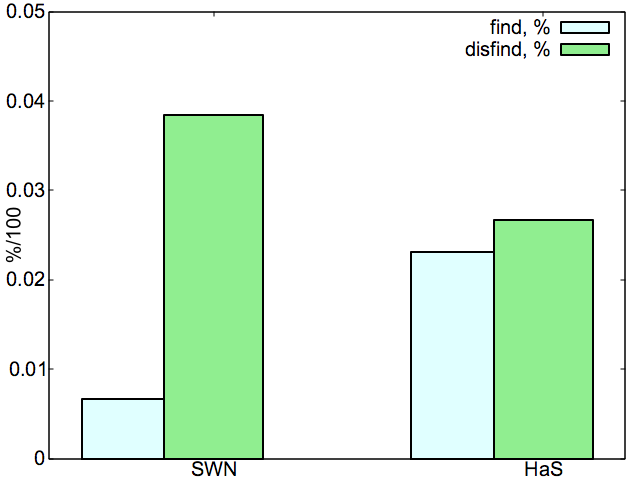
\includegraphics[width=100mm]{figures/finddisfind.png}
 \caption{ネットワークの更新によって新しくパスが見つかる確率(find)、見つからなくなる確率(disfind)}
 \label{finddisfind}
\end{figure}

\subsubsection{考察}
図\ref{finddisfind}より、スモールワールドネットワークよりハブアンドスポーク型のネットワークの方がパスを発見できるようになる確率が高く、パスが見つからなくなる確率が低いことがわかった。このことからスモールワールドネットワークよりハブアンドスポーク型の方がネットワークとして良い性質を有していると言える。当初の予想では集中ノードが生まれやすいハブアンドスポーク型の方がパスが見つからなくなる確率が高くなるのではと予想していたが、結果は逆であった。この原因として、ハブアンドスポーク型において、集中ノードになるパスが極少数であり、ランダムに辺を消す場合集中ノードが消えにくいことが考えられる。ハブアンドスポーク型において集中ノードが消えた場合にネットワーク全体に与える影響について確認しなければいけないと考える。

\subsection{実験4}
\subsubsection{実験内容}
ライトニングネットワークにおいて、ユーザは自身が所有するチャネルが支払いに使用されるたびに手数料を受け取ることができる。このことから、ユーザは自分が保有しているチャネルが使用されやすくなるように周囲のユーザと協力して他のノードにパスをつなげやすくなるように互いにチャネルを持ち合うことが考えられる。
\\
本実験ではこのチャネルを持ち合うユーザのグループを作成することでルーティングアルゴリズム全体の効率がどう変化するかを確認することを目的とする。
\par
ユーザグループはあまり大人数で作成すると\ref{sec:idea}節で述べたグローバルビーコンのようになってしまう。よってユーザグループはなるべく少人数($|V|=2000$のうち3~10人)で作成するものとする。グループの作成のため、時間$T$について前半の$[0,T/2]$についてはグループを使用しない従来の方法でパスを探索し、それまでの探索結果からグループを作成して、後半$[T/2,T]$の探索を行なった。このとき、グループを作成した場合としなかった場合でパスを発見できた確率、クエリを送信する回数がどう変化するかを確認した。
%このグループの作り方、人数を変化させながらパスを発見できる確率やクエリを送信する回数がどう変化するのかを確認した。

\subsubsection{実験結果}
グループの人数を3人とし、前半の探索の際に頻繁に使用したチャネルからグループのメンバーを選出した。このときグループの有無によりパスの発見確率、平均クエリ送信回数、グループのメンバーがRTを要求された回数がどう変化したのかを比較したものを図\ref{ex4-1}-\ref{ex4-3}に示す。

\begin{figure}[h]
 \centering
   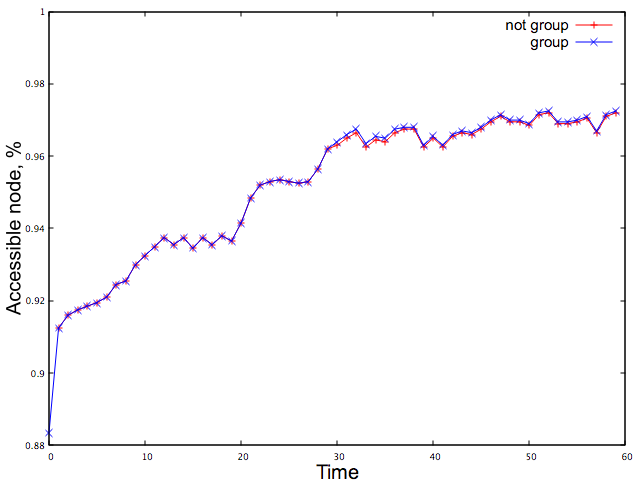
\includegraphics[width=100mm]{figures/group_accessible.png}
 \caption{パスを発見できた確率}
 \label{ex4-1}
\end{figure}

\begin{figure}[h]
 \centering
   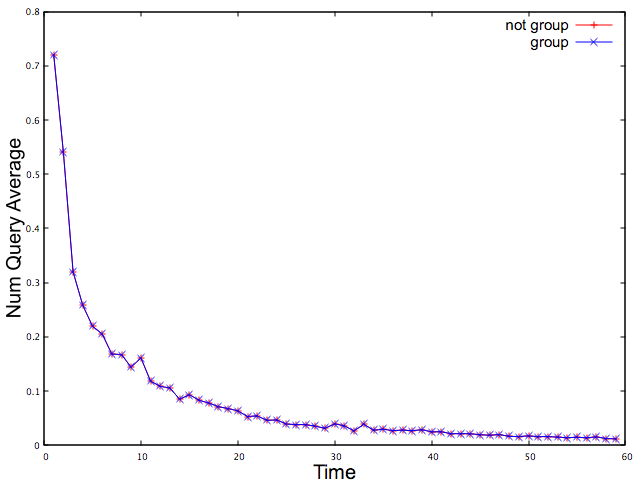
\includegraphics[width=100mm]{figures/group_query.png}
 \caption{平均クエリ送信回数}
 \label{ex4-2}
\end{figure}

\begin{figure}[h]
 \centering
   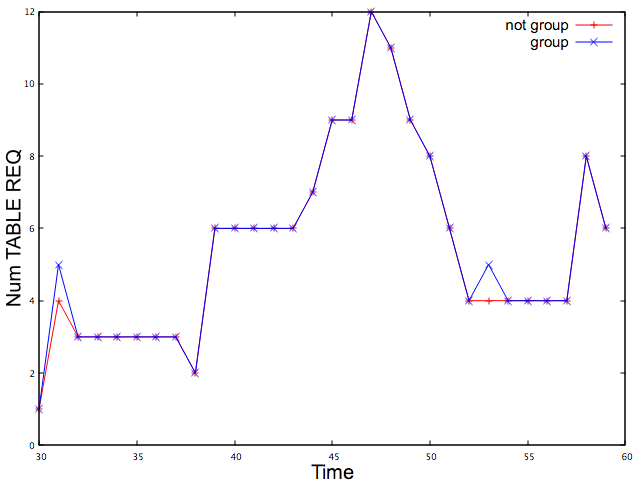
\includegraphics[width=100mm]{figures/table_req.png}
 \caption{グループメンバーがRTを要求された回数}
 \label{ex4-3}
\end{figure}

\subsubsection{考察}
現状ではグループを作成したことによるアルゴリズムのパフォーマンスへの影響は見られない。本実験で比較した3つの項目のいずれについてもグループの有無による大きな変化は確認できない。しかし、これはユーザグループをただ作成し、グラフにそれを追加しただけであり、パスを探索する際にユーザグループの存在を考慮していない。図\ref{ex4-3}においてグループの有無によってグループメンバーがRTを要求された回数に大きな差がないことから、各ノードが探索の際にRTを要求するノードは変化していないであろうことが読み取れる。ユーザグループの存在を考慮し、そのグループを優先的にビーコンとするようにアルゴリズムを拡張すれば変化があるかもしれないと考える。

\begin{thebibliography}{9}
  \bibitem{satoshi} Satoshi. Nakamoto, 2009, "Bitcoin: A Peer-to-Peer Electronic Cash System
"
  \bibitem{coin} CoinMarketCap, https://coinmarketcap.com/ja/, 2019/11/28参照
  \bibitem{joseph} Joseph. P, Thaddeus. D, 2016, "The Bitcoin Lightning Network: Scalable Off-Chain Instant Payments"
  \bibitem{jiken1} "BITPointがハッキング被害、35億円相当の仮想通貨が不正流出", 仮想通貨watch, https://crypto.watch.impress.co.jp/docs/news/1195850.html, 2019/12/3参照
  \bibitem{jiken2} "約211億円分の仮想通貨Nanoが流出。被害の取引所CEOは早々に「全額補償は不可能」とツイート", engadget, https://japanese.engadget.com/2018/02/11/211-nano-ceo/, 2019/12/3参照
  \bibitem{jiken3} "コインチェックの仮想通貨不正流出、過去最大580億円", 日本経済新聞, https://www.nikkei.com/article/DGXMZO26231090X20C18A1MM8000/, 2019/12/3参照
  \bibitem{jiken4} "仮想通貨 The DAO 事件", 仮想通貨ニュースメディアビットタイムズ, https://bittimes.net/tag/dao-attack, 2019/12/3参照
  \bibitem{security2} Arthur. G, Hubert. R, Ghassan. O. K, Srdjan. C, 2015, "Tampering with the delivery of blocks and transactions in bitcoin.", the 22nd ACM SIGSAC Conference on Computer and Communications Security, pages 692–705.
  \bibitem{security3} E. Heilman, A. Kendler, A. Zohar, S. Goldberg, 2015, "Eclipse attacks on bitcoin’s peer-to-peer network" 
  \bibitem{security4} Ghassan. O. K, Elli. A, Srdjan. C, 2012, "Double-spending fast payments in bitcoin", the 2012 ACM conference on Computer and communications security
  \bibitem{book1} 田篭 照博, 2017, 『堅牢なスマートコントラクト開発のためのブロックチェーン[技術]入門』, 株式会社技術評論社
  \bibitem{book2} 山崎 重一郎, 安土 茂亨, 田中 俊太郎, 2017, ブロックチェーン・プログラミング 仮想通貨入門, 株式会社講談社
  \bibitem{flare} Pavel. P, et al, Jun 07, 2016, “Flare: An Approach to Routing in Lightning Network”
 \bibitem{sha256} Natinal Institute of Standard and Technology(2015). Secure Hash Standard(SHS).
  \bibitem{Yen} Jin. Y. Yen, 1971, "Finding the K Shortest Loopless Paths in a Network", Management Science Vol. 17, No. 11, Theory Series (Jul., 1971), pp. 712-716
  \bibitem{swn} Duncan. J. Watts, Steven. H. Strogatz, 1998, "Collection dynamics of 'small-world' networks", In: Nature, vol. 393, pp. 440–442.
  \bibitem{idea1} Anthony. Towns, 2015, Network topology and routing. In: Lightning Network development discussion, http://lists.linuxfoundation.org/pipermail/lightning-dev/2015-September/000188.html, 2019/12/1参照
  \bibitem{idea2}Rusty. Russel, 2015, Ionization protocol: flood routing. In: Lightning Network development discussion, http://lists.linuxfoundation.org/pipermail/lightning-dev/2015-September/000199.html, 2019/12/1参照
  \bibitem{idea3} Amos. Bairn, 2015, Ionization protocol: flood routing. In: Lightning Network development discussion, http://lists.linuxfoundation.org/pipermail/lightning-dev/2015-September/000212.html, 2019/12/1参照
  \bibitem{MANET} Elizabeth. R, Chai-Keong. T, 1999. "A review of current routing protocols for ad hoc mobile wireless
networks", IEEE Personal Communications, Vol. 6 (2).
\end{thebibliography}
\end{document}
